\chapter{Parametric and Non-parametric Probabilistic Forecasting Methods Employing Deep Learning Models} \label{Unstructured} 

\section{ Motivation}
Forecasting is crucial across many fields, from energy management and finance to medicine and climatology. Accurate predictions allow stakeholders to allocate resources in turn and make intelligent choices. Traditional forecasting techniques, however, provide single-point estimates that omit uncertainty, which can lead to suboptimal or even detrimental choices, especially in high-stakes applications such as weather forecasting and financial markets. In this chapter, we aim to conduct a study on the various existing parametric and non-parametric probabilistic forecasting methods using deep learning models across a variety of datasets to assess performance using various metrics.

Probabilistic forecasting is a better option because it provides confidence intervals that allow decision-makers to plan for a range of potential outcomes and control risks. The technique, however, is not yet a widespread practice in machine learning, partly due to the lack of a shared understanding of the optimum method. While parametric techniques (e.g., Gaussian, Weibull) are simpler to apply, they might not be able to capture data complexities fully; non-parametric techniques (e.g., Quantile Regression, Bootstrap based, etc.), conversely, are more adaptable but demand more comprehensive computational resources.

Non-parametric techniques, such as the Traditional and Advanced LUBE methods, have drawn interest as well, but accuracy remains an issue compared to traditional methods. The growing significance of machine learning to probabilistic forecasting highlights the need for more research to determine the most effective methods across different applications.

Figure \ref{fig1} presents a classification of traditional probabilistic forecasting methods and Table \ref{tab:dataset_summary} represents the datasets used in this Thesis and their length.

\begin{table}[!ht]
    \caption{Summary of Datasets Used.}
    \centering
    \begin{tabular}{|p{5cm}|c|}
        \hline
        \textbf{Dataset Name} & \textbf{Length of Dataset} \\
        \hline
        \multicolumn{2}{|c|}{\textbf{Nifty50 Dataset (2000--2021)}} \\
        \hline
        Adani Ports & 3322 \\
        Asian Paints & 5306 \\
        Axis Bank & 5306 \\
        \hline
        Web Traffic & 550 \\
        Electricity Consumption & 1858 \\
        \hline
    \end{tabular}
    \label{tab:dataset_summary}
\end{table}


\section{ Methodology}
\begin{figure*}[!t]
    \centering
    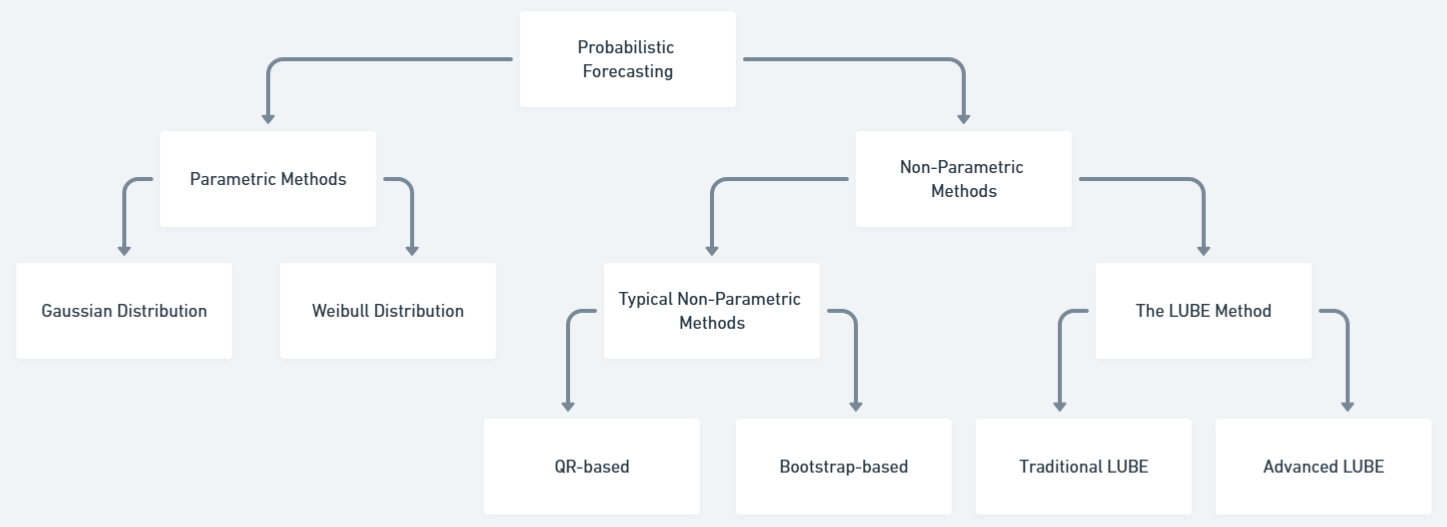
\includegraphics[width=15cm]{Chap02/Classification Of Probabilistic Methods.jpg}
    \caption{Classification of Traditional Probabilistic Methods.}
    \label{fig1}
\end{figure*}

\subsection{ Categorization Of Methods}
In this paper, six probabilistic forecasting methods are compared, broadly classified into parametric and non-parametric, each capable of producing prediction intervals (PIs) representing uncertainty in time series forecasting. Parametric methods are based on assumptions of underlying data distribution. The Gaussian (Normal) distribution-based method assumes symmetric, bell-shaped data and builds PIs from mean and standard deviation of forecast values and thus is optimal for datasets having normally distributed errors. The Weibull distribution-based method is more general and especially suited for skewed data and finds extensive use in reliability analysis and applications dealing with extreme values or variability in the data. Non-parametric methods make fewer distributional assumptions and thus find broader applicability for a wide variety of datasets. The Quantile Regression (QR)-based method estimates quantiles directly (e.g., 0.1 and 0.9 for a 90\% confidence level) to build PIs and provides robustness to non-linearity and heteroscedasticity. The Bootstrap-based method employs resampling of training data to make multiple forecasts and estimates PIs on the basis of percentiles of the resampled outputs and hence captures model and data dependent uncertainties effectively. The Traditional LUBE method builds PIs upon a custom loss function to reduce interval width and ensure adequate coverage, trading off tightness and reliability of intervals. The Advanced LUBE method builds on this by optimizing performance using novel metrics like Absolute Coverage Error (ACE) and Absolute Width Error (AWE), providing more robustness to outliers and stability at multiple confidence levels. These methods, collectively, provide a comprehensive probabilistic forecasting framework under a wide range of data conditions and uncertainty profiles.

\subsection{ Deep Learning Models}
To implement the aforementioned probabilistic forecasting techniques, four deep learning models were utilized: Long Short-Term Memory (LSTM), Gated Recurrent Unit (GRU), Convolutional Neural Network (CNN) and Bidirectional LSTM (BiLSTM). LSTM is a recurrent neural networks (RNNs) architecture specifically developed to learn long term temporal relationships in sequential data and is hence well suited for time series with intricate temporal patterns. GRU is a compact version of LSTM and hence possesses similar capabilities but lower computational complexity and is thus suitable for applications with low memory demands. CNNs, while initially developed for spatial data, have been used successfully for time series by encoding temporal sequences as structured inputs, allowing strong feature extraction through localized pattern detection. BiLSTM is an extension of LSTM with the ability to process input sequences in both directions and hence extract contextual information from past and future time steps for enhanced forecasting accuracy. These architectures were chosen based on their proven efficiency in time series forecasting tasks and their compatibility with both parametric and non-parametric probabilistic techniques.


\subsection{ Methodology}
\begin{itemize}
    \item \textbf{Dataset Preparation}
    In all the approaches described in the present study, the data preparation was performed consistently. Five different datasets were used, three stock price datasets of Nifty50 Dataset (2000-2021): Adani Ports, Asian Paints and Axis Bank and two other datasets: the Electricity Consumption dataset and the Web Traffic dataset \ref{tab:dataset_summary}. The respective target variables for prediction were 'VWAP' for the stock price datasets, 'Consumption' for the electricity dataset, and 'Views' for the web traffic dataset. The target variables were normalized first with Min-Max Scaling to provide stable convergence of the models. Next, a sliding window technique was employed to transform the time series data into a supervised learning format, thus generating several input-output pairs suitable for model training. The generated records were divided equally into training, validation, and test sets using a 70:15:15 ratio for all experimental protocols.

    \item \textbf{Evaluation Metrics}
    In this thesis, we have used the following Evaluation Metrics for fair comparison across all the methods:\\
    1. PICP (Prediction Interval Coverage Probability):\\
    Quantifies the proportion of actual values that are contained within the defined prediction intervals.
    \begin{equation}
    \begin{aligned}
    \text{PICP} = \frac{\text{Number of samples where } LB_i \leq y_i \leq UB_i}{n}
    \end{aligned}
    \label{Equation 1}
    \end{equation}
    Where:\\ 
    $y_i$: The actual observed value at time step $i$.\\
    $LB_i$: The predicted \textbf{lower bound} of the prediction interval at time step $i$.\\
    $UB_i$: The predicted \textbf{upper bound} of the prediction interval at time step $i$.\\ \\
    2. PINAW (Prediction Interval Normalized Average Width):\\
    This metric assesses the precision of the intervals.
    \begin{equation}
    \begin{aligned}
    \text{PINAW} = \frac{\frac{1}{n} \sum_{i=1}^n (UB_i - LB_i)}{\max(y) - \min(y)}
    \end{aligned}
    \label{Equation 2}
    \end{equation}
    Where:\\ 
    $n$: Total number of forecasted data points or time steps.\\
    $\max(y)$, $\min(y)$: The maximum and minimum values of the observations $y_i$ across all $n$ samples. These are used to normalize the interval width in PINAW.
    \\ \\
    3. ACE (Absolute Coverage Error):\\
    Defines the difference between actual coverage and nominally assumed confidence.
    \begin{equation}
    \begin{aligned}
    \text{ACE} = |\text{PICP} - c|
    \end{aligned}
    \label{Equation 3}
    \end{equation}
    Where $c$: The nominal confidence level of the prediction interval (e.g., 0.90 for a 90\% confidence interval).
    \\ \\
    4. AWE (Average Weighted Error):\\
    PICP and PINAW combined into an evaluation metric that is weighted.
    \begin{equation}
    \begin{aligned}
    \text{AWE} = \left| \frac{1}{n} \sum_{i=1}^n (UB_i - LB_i) - (\max(y) - \min(y)) \right|
    \end{aligned}
    \label{Equation 4}
    \end{equation}
    \\

    Eq. \eqref{Equation 1} represents the PICP evaluation metric, Eq. \eqref{Equation 2} represents the PINAW evaluation metric, Eq. \eqref{Equation 3} represents the ACE evaluation metric and finally Eq. \eqref{Equation 4} represents the AWE evaluation metric. These four metrics is used throughout this thesis to compare and evaluate perfromance of the different methods.

    \item \textbf{Output Generation}
    For every forecasting technique used, the resulting predicted intervals, performance metrics and mean results are systematically arranged in CSV file format for further evaluation and reproducibility. Visual verification is executed by generating graphs displaying the prediction intervals at different confidence levels (0.9, 0.8, 0.7, 0.6) with the actual values plotted alongside the corresponding interval boundaries. These visual graphs play a critical role in ascertaining the coverage and validity of the intervals. In addition, comparative plots are generated for every deep learning model i.e., LSTM, GRU, CNN and BiLSTM such that predictive accuracy as well as uncertainty estimation can be visually compared for the different probabilistic forecasting techniques. (These graphs are present in Figures \ref{Fi 3.2} to \ref{Fi 3.7}). The Tables \ref{Table 1} to \ref{Table 10} displays the performances of all the methods used across the five different datasets.

    
    \subsubsection{Probabilistic Forecasting Using Traditional LUBE Method}
        This algorithm describes the Traditional LUBE method that trains deep learning networks (LSTM, CNN, GRU, BiLSTM) directly through a custom loss function that is given below in Eq. \eqref{Lube Loss} consisting of lower and upper pinball loss as in Eq. \eqref{Loss Lower} and Eq. \eqref{Loss Upper} and a coverage penalty to produce interval boundaries independent of distributional assumptions. A few equations essential to compute Lube Loss is given below:\\
        
        \begin{equation}
            \text{Loss}_{\text{lower}} = \frac{1}{n} \sum \max(0, LB_i - y_i) \cdot q
            \label{Loss Lower}
        \end{equation}

        \begin{equation}
            \text{Loss}_{\text{upper}} = \frac{1}{n} \sum \max(0, y_i - UB_i) \cdot (1 - q)
        \label{Loss Upper}
        \end{equation}

        \begin{equation}
        \text{Loss}_{\text{LUBE}} = \text{Loss}_{\text{lower}} + \text{Loss}_{\text{upper}} + \lambda \max(0.9 - \text{PICP}, 0)^2
        \label{Lube Loss}
        \end{equation}

        Where:
        \begin{itemize}
        \item $y_i$: Actual (true) value of the $i$-th sample
        \item $LB_i$: Predicted lower bound of the prediction interval for the $i$-th sample
        \item $UB_i$: Predicted upper bound of the prediction interval for the $i$-th sample
        \item $n$: Total number of samples
        \item $q$: Quantile level (e.g., $0.1$ for $90\%$ prediction interval)
        \item $\lambda$: Regularization parameter controlling the penalty for low coverage in the LUBE loss function
        \end{itemize}
        
        \begin{algorithm}[H]
        \footnotesize
        %\normalsize
        \SetAlgoNlRelativeSize{0}
        \SetAlgoCaptionSeparator{:}
        
        \KwIn{Time series dataset $D$}
        \KwOut{Predicted intervals $[LB, UB]$, PICP, PINAW, ACE, AWE}
        
        \textbf{Step 1: Data Preprocessing}\\
        Normalize $D$ using MinMaxScaler\\
        Generate input-output pairs with window size $w$\\
        Split into train, validation, and test sets\\
        
        \textbf{Step 2: Define LUBE Loss}\\
        \ForEach{$c \in \{0.9, 0.8, 0.7, 0.6\}$}{
            $q = 1 - c$\\
            Compute $LB$, $UB$\\
            Compute $\text{Loss}_{\text{lower}}$ (as in Eq. \eqref{Loss Lower}) and $\text{Loss}_{\text{upper}}$ (as in Eq. \eqref{Loss Upper})\\
            Compute \text{PICP} = \text{(as in Eq. \eqref{Equation 1})}\\
            Compute $\text{Loss}_{\text{LUBE}}$ (as in Eq. \eqref{Lube Loss})
        }
        
        \textbf{Step 3: Model Training}
        \ForEach{$M \in \{$LSTM, CNN, GRU, BiLSTM$\}$}{
            Define model architecture\\
            Compile with LUBE loss\\
            Train on $(X_{\text{train}}, y_{\text{train}})$ for $e$ epochs\\
            Validate on $(X_{\text{val}}, y_{\text{val}})$\\
            Save $LB, UB$ for test data
        }
        
        \textbf{Step 4: Evaluation Metrics} Compute the PINAW (as in Eq. ~\eqref{Equation 2}), ACE (as in Eq. ~\eqref{Equation 3}) and AWE (as in Eq. ~\eqref{Equation 4}) of the computed prediction intervals.
        
        \textbf{Step 5: Aggregate Results}\\
        Compute mean of metrics for all models
        
        \caption{Traditional LUBE Method.}
        \end{algorithm}
 
        The Traditional LUBE (Lower Upper Bound Estimation) Method Algorithm is designed to generate reliable prediction intervals for time series forecasting using deep learning models. The process begins with data pre-processing, where the input time series is normalized using MinMaxScaler and transformed into input-output pairs based on a sliding window of size $w$, followed by splitting the dataset into training, validation, and test sets. A custom LUBE loss function is defined for different confidence levels $c \in \{0.9, 0.8, 0.7, 0.6\}$, where the loss penalizes predictions falling outside the predicted lower ($LB$) and upper ($UB$) bounds and encourages higher coverage through a PICP-based regularization term. For each selected deep learning model (LSTM, CNN, GRU, BiLSTM), the model is compiled using the LUBE loss and trained on the preprocessed data. The predicted bounds on the test set are evaluated using four key probabilistic metrics: Prediction Interval Coverage Probability (PICP), Prediction Interval Normalized Average Width (PINAW), Average Coverage Error (ACE), and Average Width Error (AWE). Finally, the algorithm aggregates the results across all models, computing the mean and standard deviation of each evaluation metric, thereby offering a robust assessment of the interval prediction performance.


    \subsubsection{Probabilistic Forecasting using Advance LUBE Method}
        This algorithm describes The Advanced LUBE method that enhances this Traditional LUBE method by introducing an extra regularization term controlled by hyperparameter $\mu$ which applies penalties on wide intervals to improve sharpness.\\
        The Advanced LUBE Loss Function is given below in Eq. \eqref{Advanced Lube Loss}.
        \begin{equation}
            \text{Loss}_{\text{LUBE}} = \text{Loss}_{\text{upper}} + \lambda \max(0.9 - \text{PICP}, 0)^2 + \mu \cdot \frac{1}{n} \sum |UB_i - LB_i|
        \label{Advanced Lube Loss}
        \end{equation}

        Where:
        \begin{itemize}
        \item $\text{Loss}_{\text{upper}}$: Penalty for true values exceeding the upper bound of the prediction interval. (Given in Eq. \eqref{Loss Upper})
        \item $UB_i$: Predicted upper bound for the $i$-th sample
        \item $LB_i$: Predicted lower bound for the $i$-th sample
        \item $n$: Total number of samples
        \item $\lambda$: Regularization parameter penalizing insufficient coverage
        \item $\mu$: Regularization parameter controlling the width of the prediction interval
        \item $\max(0.9 - \text{PICP}, 0)^2$: Coverage penalty term encouraging the model to achieve at least 90\% PICP
        \item $\sum |UB_i - LB_i|$: Total width of the prediction intervals across all samples
        \end{itemize}


        \begin{algorithm}[H]
        \footnotesize
        %\normalsize
        \SetAlgoNlRelativeSize{0}
        \SetAlgoCaptionSeparator{:}
    
        \KwIn{Time series dataset $D$}
        \KwOut{Predicted intervals $[LB, UB]$, PICP, PINAW, ACE, AWE}
    
        \textbf{Step 1: Data Preprocessing}\\
        Normalize $D$ using MinMaxScaler\\
        Generate input-output pairs with window size $w$\\
        Split into train, validation, and test sets
    
        \textbf{Step 2: Define Advanced LUBE Loss}\\
        \ForEach{$c \in \{0.9, 0.8, 0.7, 0.6\}$}{
            $q = 1 - c$\\
            Compute $LB$, $UB$\\
            Compute $\text{Loss}_{\text{lower}}$ (as in Eq. \eqref{Loss Lower}) and $\text{Loss}_{\text{upper}}$ (as in Eq. \eqref{Loss Upper})\\
            Compute PICP and PINAW (as in Eq. \eqref{Equation 1} and \eqref{Equation 2} respectively)\\
            Compute $\text{Loss}_{\text{LUBE}}$ (as in Eq. \eqref{Advanced Lube Loss})
        }
    
        \textbf{Step 3: Model Training}\\
        \ForEach{$M \in \{$LSTM, CNN, GRU, BiLSTM$\}$}{
            Define model architecture\\
            Compile with Advanced LUBE loss\\
            Train on $(X_{\text{train}}, y_{\text{train}})$ for $e$ epochs\\
            Validate on $(X_{\text{val}}, y_{\text{val}})$\\
            Save $LB, UB$ for test data
        }
    
        \textbf{Step 4: Evaluation Metrics}\\
        Compute ACE (as in Eq. \eqref{Equation 3}) and AWE (as in Eq. \eqref{Equation 4})
    
        \textbf{Step 5: Aggregate Results}\\
        Compute mean of metrics for all models and confidence levels
        
        \caption{Advanced LUBE Method.}
        \end{algorithm}

        The Advanced LUBE Method Algorithm enhances the traditional LUBE framework by incorporating interval width regularization into the loss function, thereby promoting both accuracy and tightness of prediction intervals. The process begins with data pre-processing where the time series dataset is normalized using MinMaxScaler, transformed into input-output pairs using a sliding window of size $w$, and divided into training, validation, and test subsets. The advanced LUBE loss function is defined for multiple confidence levels $c \in \{0.9, 0.8, 0.7, 0.6\}$, with penalties for predictions outside the bounds and additional terms for poor coverage (via PICP) and overly wide intervals (via PINAW). Specifically, the loss includes a regularization term proportional to the average width of the intervals, controlled by the hyperparameter $\mu$. For each deep learning model (LSTM, CNN, GRU, BiLSTM), the model is trained using this advanced loss formulation. The predicted intervals are evaluated using standard probabilistic metrics including PICP, PINAW, Average Coverage Error (ACE), and Average Width Error (AWE). Finally, the results across all models and confidence levels are aggregated to compute the mean and standard deviation of each metric, offering a robust and comprehensive assessment of the method’s performance.


    \subsubsection{Probabilistic Forecasting using QR-based Method}
    This algorithm describes the Quantile Regression based algorithm that uses quantile loss functions to estimate lower and upper quantiles, summing pinball losses and under-coverage penalties and hence providing statistically well-motivated alternatives to LUBE methods. The following equations are needed to construct the QR Loss Function. Eq. \eqref{q lower} shows the Lower quantile threshold while Eq. \eqref{q upper} shows the Upper Quantile threshold. Eq. \eqref{loss_lower} and \eqref{loss_upper} calculates the Lower and Upper losses, i.e Penalty for predicted lower or upper bounds exceeding or under flowing true values. Finally, Eq. \eqref{loss_qr} shows the QR Loss function. \\

    \begin{equation}
        q_{\text{lower}} = \frac{1 - c}{2}
        \label{q lower}
    \end{equation}

    \begin{equation}
        q_{\text{upper}} = 1 - q_{\text{lower}}
        \label{q upper}
    \end{equation}

    \begin{equation}
    \text{Loss}_{\text{lower}} = \frac{1}{n} \sum \max(0, LB_i - y_i) \cdot q_{\text{lower}}
    \label{loss_lower}
    \end{equation}
    
    \begin{equation}
    \text{Loss}_{\text{upper}} = \frac{1}{n} \sum \max(0, y_i - UB_i) \cdot q_{\text{upper}}
    \label{loss_upper}
    \end{equation}

    \begin{equation}
    \text{Loss}_{\text{QR}} = \text{Loss}_{\text{lower}} + \text{Loss}_{\text{upper}} + \lambda \cdot \max(0.9 - \text{PICP}, 0)^2 + \mu \cdot \frac{1}{n} \sum |UB_i - LB_i|
    \label{loss_qr}
    \end{equation}

    Where:
    \begin{itemize}
    \item $c$ – Confidence level (e.g: 0.9, 0.8, 0.7 and 0.6)
    \item $q_{\text{lower}}$ – Lower quantile threshold.
    \item $q_{\text{upper}}$ – Upper quantile threshold.
    \item $LB_i$ – Predicted lower bound of the $i$-th interval
    \item $UB_i$ – Predicted upper bound of the $i$-th interval
    \item $y_i$ – Actual target value at index $i$
    \item $n$ – Total number of samples
    \item $\text{Loss}_{\text{lower}}$ – Penalty for predicted lower bounds exceeding true values.
    \item $\text{Loss}_{\text{upper}}$ – Penalty for predicted upper bounds below true values.
    \item $\lambda$ – Penalty coefficient for inadequate coverage
    \item $\mu$ – Penalty coefficient for interval width
    \item $\text{PICP}$ – Prediction Interval Coverage Probability
    \item $\text{Loss}_{\text{QR}}$ – Total quantile regression-based loss function.
    \end{itemize}

        \begin{algorithm}[H]
        \footnotesize
        %\normalsize
        \SetAlgoNlRelativeSize{0}
        \SetAlgoCaptionSeparator{:}
    
        \KwIn{Time series dataset $D$}
        \KwOut{Predicted intervals $[LB, UB]$, PICP, PINAW, ACE, AWE}
    
        \textbf{Step 1: Data Preprocessing}\\
        Normalize $D$ using MinMaxScaler\\
        Generate input-output pairs with window size $w$\\
        Split into train, validation, and test sets
    
        \textbf{Step 2: Define QR Loss Function}\\
        \ForEach{$c \in \{0.9, 0.8, 0.7, 0.6\}$}{
            Compute $q_{\text{lower}}$ (as in Eq.~\eqref{q lower}) and $q_{\text{upper}}$ (as in Eq.~\eqref{q upper})\\
            Compute $LB$, $UB$\\
            Compute $Loss_{\text{lower}}$ (as in Eq. \eqref{loss_lower}) and $Loss_{\text{upper}}$ (as in Eq. \eqref{loss_upper})\\
            Compute PICP (as in Eq.\eqref{Equation 1}) and PINAW (as in Eq. \eqref{Equation 2})\\
            Compute $Loss_{\text{QR}}$ (as in Eq. \eqref{loss_qr})
        }
    
        \textbf{Step 3: Model Training}\\
        \ForEach{$M \in \{$LSTM, CNN, GRU, BiLSTM$\}$}{
            Define model architecture\\
            Compile with QR-based loss\\
            Train on $(X_{\text{train}}, y_{\text{train}})$ for $e$ epochs\\
            Validate on $(X_{\text{val}}, y_{\text{val}})$\\
            Save $LB, UB$ for test data
        }
    
        \textbf{Step 4: Evaluation Metrics}\\
        Compute ACE (as in \eqref{Equation 3} and AWE (as in Eq. \eqref{Equation 4})
    
        \textbf{Step 5: Aggregate Results}\\
        Compute mean of metrics for all models and confidence levels
    
        \caption{Quantile Regression (QR)-based Method.}
        \end{algorithm}

        The Quantile Regression (QR)-based Method Algorithm applies quantile regression principles to construct asymmetric prediction intervals for time series forecasting. Initially, the time series dataset is normalized using MinMaxScaler, and transformed into supervised input-output pairs using a sliding window of size $w$, followed by splitting into training, validation, and testing subsets. For each confidence level $c \in \{0.9, 0.8, 0.7, 0.6\}$, the algorithm calculates the lower and upper quantiles as $q_{\text{lower}} = \frac{1 - c}{2}$ and $q_{\text{upper}} = 1 - q_{\text{lower}}$, which define the predicted interval bounds $[LB, UB]$. The QR loss function combines penalties for underestimation and overestimation, weighted by their respective quantiles. Additional terms for improving interval quality include a PICP regularization component and a width regularization term, scaled by hyperparameters $\lambda$ and $\mu$. Deep learning models (LSTM, CNN, GRU, BiLSTM) are then trained using this composite loss. The performance of each model is assessed using PICP, PINAW, Average Coverage Error (ACE), and Average Width Error (AWE). Finally, results across all models and confidence levels are aggregated by computing the mean and standard deviation of each metric, ensuring a comprehensive evaluation of the prediction interval reliability and efficiency.


    \subsubsection{Probabilistic Forecasting using Bootstrap-based Method}
    This algorithm describes the Bootstrap-Based method that estimates uncertainty by training models over multiple resampled datasets and estimating empirical prediction intervals from the predictions ensemble, and this provides it with robustness without assuming a residual distribution.\\
        
        \begin{algorithm}[H]
        \footnotesize
        %\normalsize
        \SetAlgoNlRelativeSize{0}
        \SetAlgoCaptionSeparator{:}
    
        \KwIn{Time series dataset $D$}
        \KwOut{Predicted intervals $[LB, UB]$, PICP, PINAW, ACE, AWE}
    
        \textbf{Step 1: Data Preprocessing}\\
        Normalize $D$ using MinMaxScaler\\
        Generate input-output pairs with window size $w$\\
        Split into train, validation, and test sets
    
        \textbf{Step 2: Bootstrap Prediction Intervals}\\
        \ForEach{$c \in \{0.9, 0.8, 0.7, 0.6\}$}{
            Generate $B$ bootstrap samples from training data\\
            \ForEach{bootstrap sample}{
                Train model $M$ and predict on test set
            }
            \ForEach{test sample $y_{\text{test}}^i$}{
                Compute $LB_i$ and $UB_i$ as empirical quantiles at $q_{\text{lower}}$ and  $q_{\text{upper}}$ as in Eq. \eqref{q lower} and \eqref{q upper}
            }
        }
    
        \textbf{Step 3: Evaluation Metrics} Compute the PICP (as in Eq.~\eqref{Equation 1}), PINAW (as in Eq. ~\eqref{Equation 2}), ACE (as in Eq. ~\eqref{Equation 3}) and AWE (as in Eq. ~\eqref{Equation 4}) of the computed prediction intervals.
    
        \textbf{Step 4: Aggregate Results}\\
        Compute mean of metrics for all models and confidence levels
    
        \caption{Bootstrap-based Method.}
        \end{algorithm}

        The Bootstrap-Based Method Algorithm leverages the statistical resampling technique of bootstrapping to generate robust prediction intervals for time series forecasting. The procedure begins with data pre-processing, where the dataset is normalized using MinMaxScaler, converted into input-output pairs using a sliding window of size $w$, and partitioned into training, validation, and testing subsets. For each confidence level $c \in \{0.9, 0.8, 0.7, 0.6\}$, $B$ bootstrap samples are generated from the training data. A deep learning model $M$ (e.g., LSTM, CNN, GRU, BiLSTM) is trained on each sample and used to generate predictions on the test set. For each test instance, the lower and upper bounds of the prediction interval ($LB_i$ and $UB_i$) are computed as empirical quantiles corresponding to $q_{\text{lower}} = \frac{1 - c}{2}$ and $q_{\text{upper}} = 1 - q_{\text{lower}}$ from the bootstrap distribution. The intervals are evaluated using probabilistic forecasting metrics: Prediction Interval Coverage Probability (PICP), Prediction Interval Normalized Average Width (PINAW), Average Coverage Error (ACE), and Average Width Error (AWE). The final step aggregates the performance metrics across all models and confidence levels by computing their mean and standard deviation, thereby providing a comprehensive assessment of interval reliability and sharpness.


    \subsubsection{Probabilistic Forecasting using Gaussian Distribution based Method}
    This algorithm uses the target variable as normally distributed and computes symmetric intervals around the mean using standard normal distribution z-scores, providing it with ease of implementation but lack of flexibility in dealing with non-Gaussian datasets. Eq. \eqref{z_score} provides the Z-score while Eq. \eqref{low_bound} and Eq. \eqref{up_bound} provides the Lower and Upper bounds of the prediction interval.\\

    \begin{equation}
    z_c = \Phi^{-1}\left(\frac{1 + c}{2}\right)
    \label{z_score}
    \end{equation}

    \begin{equation}
        LB = \mu - z_c \cdot \sigma
    \label{low_bound}
    \end{equation}

    \begin{equation}
        UB = \mu + z_c \cdot \sigma
        \label{up_bound}
    \end{equation}

    Where:
    \begin{itemize}
        \item $c$: Confidence level (e.g., 0.9 for 90\% confidence)
        \item $\Phi^{-1}$: Inverse cumulative distribution function (quantile function) of the standard normal distribution.
        \item $z_c$: Z-score corresponding to the confidence level $c$.
        \item $\mu$: Mean (expected value) of the distribution.
        \item $\sigma$: Standard deviation of the distribution.
        \item $LB$: Lower bound of the prediction interval.
        \item $UB$: Upper bound of the prediction interval.
    \end{itemize}


        \begin{algorithm}[H]
        \footnotesize
        %\normalsize
        \SetAlgoNlRelativeSize{0}
        \SetAlgoCaptionSeparator{:}
    
        \KwIn{Time series dataset $D$ with target variable $y$}
        \KwOut{Predicted intervals $[LB, UB]$, PICP, PINAW, ACE, AWE}
    
        \textbf{Step 1: Data Preprocessing}\\
        Remove missing values to obtain cleaned target $y$
    
        \textbf{Step 2: Define Confidence Levels}\\
        $C = \{0.9, 0.8, 0.7, 0.6\}$
    
        \textbf{Step 3: Estimate Distribution Parameters}\\
        Compute mean $\mu$ and standard deviation $\sigma$ of $y$
    
        \textbf{Step 4: Generate Prediction Intervals}\\
        \ForEach{$c \in C$}{
            Compute $z_c$ (as in Eq. \eqref{z_score})
            Compute LB as in Eq. \eqref{low_bound} and UB as in Eq. \eqref{up_bound}
        }
    
        \textbf{Step 5: Evaluation Metrics} Compute the PICP (as in Eq.~\eqref{Equation 1}), PINAW (as in Eq. ~\eqref{Equation 2}), ACE (as in Eq. ~\eqref{Equation 3}) and AWE (as in Eq. ~\eqref{Equation 4}) of the computed prediction intervals.
    
        \caption{Gaussian Distribution based Method.}
        \end{algorithm}
        The Gaussian Distribution-Based Method Algorithm estimates prediction intervals under the assumption that the target variable follows a normal distribution. The algorithm begins by pre-processing the time series data $D$ to remove missing values, producing a clean target variable $y$. It then defines a set of confidence levels $C = \{0.9, 0.8, 0.7, 0.6\}$ for interval estimation. For each confidence level $c \in C$, the algorithm calculates the corresponding $z$-score using the inverse cumulative distribution function $\Phi^{-1}$. Using the mean $\mu$ and standard deviation $\sigma$ of the target variable, the lower and upper bounds of the prediction interval are computed as $LB = \mu - z_c \cdot \sigma$ and $UB = \mu + z_c \cdot \sigma$, respectively. The intervals are then evaluated using standard probabilistic metrics: Prediction Interval Coverage Probability (PICP), Prediction Interval Normalized Average Width (PINAW), Average Coverage Error (ACE), and Average Width Error (AWE). Finally, the method aggregates and stores the computed intervals and corresponding metric values for each confidence level, providing a baseline assessment of uncertainty using parametric Gaussian assumptions.



    \subsubsection{Probabilistic Forecasting Weibull Distribution based Method}
    This algorithm describes the Weibull Distribution method that employs a fitted Weibull distribution by maximum likelihood to model the target, facilitating interval estimation with the percent point function and showing better compliance with skewed or heavy-tailed data sets. Eq. \eqref{eq:alpha} shows the Tail Probability. Eq. \eqref{eq:weibull_lb} and Eq. \eqref{eq:weibull_ub} shows the formulae for UB and LB calculation of Prediction Intervals. \\

    \begin{equation}
        \alpha = \frac{1 - c}{2}
        \label{eq:alpha}
    \end{equation}

    \begin{equation}
        LB = \text{PPF}(\alpha, \kappa, \lambda)
        \label{eq:weibull_lb}
    \end{equation}
    
    \begin{equation}
        UB = \text{PPF}(1 - \alpha, \kappa, \lambda)
        \label{eq:weibull_ub}
    \end{equation} 

    Where:
    \vspace{0.5cm}
    \begin{itemize}
        \item $c$ — Confidence level (e.g., 0.6, 0.7, 0.8, or 0.9) used to construct the prediction interval.
        \item $\alpha$ — Tail probability, representing the area in each tail of the distribution outside the prediction interval.
        \item $\text{PPF}$ — Percent-Point Function (inverse of the CDF), used to obtain the value (quantile) corresponding to a given cumulative probability from the Weibull distribution.
        \item $\kappa$ — Shape parameter of the Weibull distribution.
        \item $\lambda$ — Scale parameter of the Weibull distribution.
        \item $LB$ — Lower bound of the prediction interval, derived from the $\alpha$ quantile of the Weibull distribution.
        \item $UB$ — Upper bound of the prediction interval, derived from the $(1 - \alpha)$ quantile of the Weibull distribution.
    \end{itemize}

    
        \begin{algorithm}[H]
        \footnotesize
        %\normalsize
        \SetAlgoNlRelativeSize{0}
        \SetAlgoCaptionSeparator{:}
    
        \KwIn{Time series dataset $D$ with target variable $y$}
        \KwOut{Predicted intervals $[LB, UB]$, PICP, PINAW, ACE, AWE}
    
        \textbf{Step 1: Data Preprocessing}\\
        Remove missing values to obtain cleaned target $y$
    
        \textbf{Step 2: Define Confidence Levels}\\
        $C = \{0.9, 0.8, 0.7, 0.6\}$
    
        \textbf{Step 3: Estimate Weibull Parameters}\\
        Fit Weibull distribution to $y$ using Maximum Likelihood Estimation (MLE)\\
        Obtain shape $\kappa$, scale $\lambda$, and location $\theta$ (fixed to 0)
    
        \textbf{Step 4: Generate Prediction Intervals}\\
        \ForEach{$c \in C$}{
            Compute $\alpha$ (as in Eq. \eqref{eq:alpha})\\
            Compute LB (as in Eq. \eqref{eq:weibull_lb}) and UB (as in Eq. \eqref{eq:weibull_ub})
        }
    
        \textbf{Step 5: Evaluation Metrics} Compute the PICP (as in Eq.~\eqref{Equation 1}), PINAW (as in Eq. ~\eqref{Equation 2}), ACE (as in Eq. ~\eqref{Equation 3}) and AWE (as in Eq. ~\eqref{Equation 4}) of the computed prediction intervals.
        \caption{Weibull Distribution based Method.}
        \end{algorithm}

        The Weibull Distribution-Based Method Algorithm models uncertainty in time series forecasting by fitting a Weibull distribution to the target variable. Initially, the dataset $D$ undergoes pre-processing to remove missing values, yielding a clean target $y$. The method then defines a set of confidence levels $C = \{0.9, 0.8, 0.7, 0.6\}$ for probabilistic prediction. Using Maximum Likelihood Estimation (MLE), the Weibull distribution is fitted to $y$ to estimate its shape parameter $\kappa$, scale parameter $\lambda$, and a fixed location parameter $\theta = 0$. For each confidence level $c \in C$, the method computes the lower and upper prediction bounds as the $\alpha$ and $1-\alpha$ percentiles from the Weibull percent point function (PPF). These prediction intervals are assessed using four standard metrics: Prediction Interval Coverage Probability (PICP), Prediction Interval Normalized Average Width (PINAW), Average Coverage Error (ACE) and Average Width Error (AWE). Finally, the algorithm stores the intervals and corresponding metric values across all defined confidence levels, offering a flexible, non-Gaussian parametric approach to interval forecasting.

\end{itemize}
All the six algorithms start with typical data preprocessing tasks, including normalization using MinMaxScaler and time series data transformation to input-output pairs using a sliding window approach. Each algorithm is set up to produce prediction intervals for different confidence levels (90\%, 80\%, 70\%, 60\%) and is compared to measures like Prediction Interval Coverage Probability (PICP), Prediction Interval Normalized Average Width (PINAW), Absolute Coverage Error (ACE) and Average Width Error (AWE), and their results are logged and plotted to compare against. 
\\ Overall, the collection of algorithms provides a diverse array of methods for probabilistic time series forecasting, balancing model-driven learning with statistical as well as distributional methods.

\section{ Results and Discussions}

This section displays the evaluation of the six different parametric and non-parametric methods across five datasets. The performance of each method is assessed using metrics PICP, PINAW, ACE and AWE. The results are visualized through prediction interval plots and summarized in tables.

Figure \ref{Fi 3.2} shows Prediction Intervals for Adani Ports dataset obtained using Advanced LUBE and (a) BiLSTM, (b) CNN, (c) GRU, (d) LSTM Models.
Figure \ref{Fi 3.3} shows Prediction Intervals for Asian Paints dataset obtained using Traditional LUBE and (a) BiLSTM, (b) CNN, (c) GRU, (d) LSTM Models.
Figure \ref{Fi 3.4} shows Prediction Intervals for Axis Bank dataset obtained using QR-based method and (a) BiLSTM, (b) CNN, (c) GRU, (d) LSTM Models.
Figure \ref{Fi 3.5} shows Prediction Intervals for Electricity Consumption dataset obtained using Bootstrap-based method and (a) BiLSTM, (b) CNN, (c) GRU, (d) LSTM Models.
Figures \ref{Fi 3.6} and \ref{Fi 3.7} shows Prediction Intervals for (a) Adani Ports, (b) Asian Paints, (c) Axis Bank, (d) Electricity Consumption Load, (e) Web Traffic datasets obtained using Gaussian Distribution and Weibull Distribution based methods respectively.

Tables \ref{Table 1}, \ref{Table 2}, \ref{Table 3}, \ref{Table 4} and \ref{Table 5} shows the comparative performance of Traditional LUBE, Advanced LUBE, QR-based and Bootstrap-based methods on metrics PICP, PINAW, ACE and AWE across multiple confidence levels (90\%, 80\%, 70\% and 60\%) using four DL Models BiLSTM, CNN, GRU and LSTM obtained on Adani Ports, Asian Paints, Axis Bank, Electricity Consumption and Web Traffic datasets respectively whereas Tables \ref{Table 6}, \ref{Table 7}, \ref{Table 8}, \ref{Table 9} and \ref{Table 10} shows the performance of Gaussian Distribution and Weibull Distribution on metrics PICP, PINAW, ACE and AWE across multiple confidence levels (90\%, 80\%, 70\% and 60\%) obtained on Adani Ports, Asian Paints, Axis Bank, Electricity Consumption and Web Traffic datasets respectively.


\begin{figure}[H]
    \centering
        \begin{minipage}{0.6\textwidth}
            \centering
            \begin{subfigure}[b]{\textwidth}
                \centering
                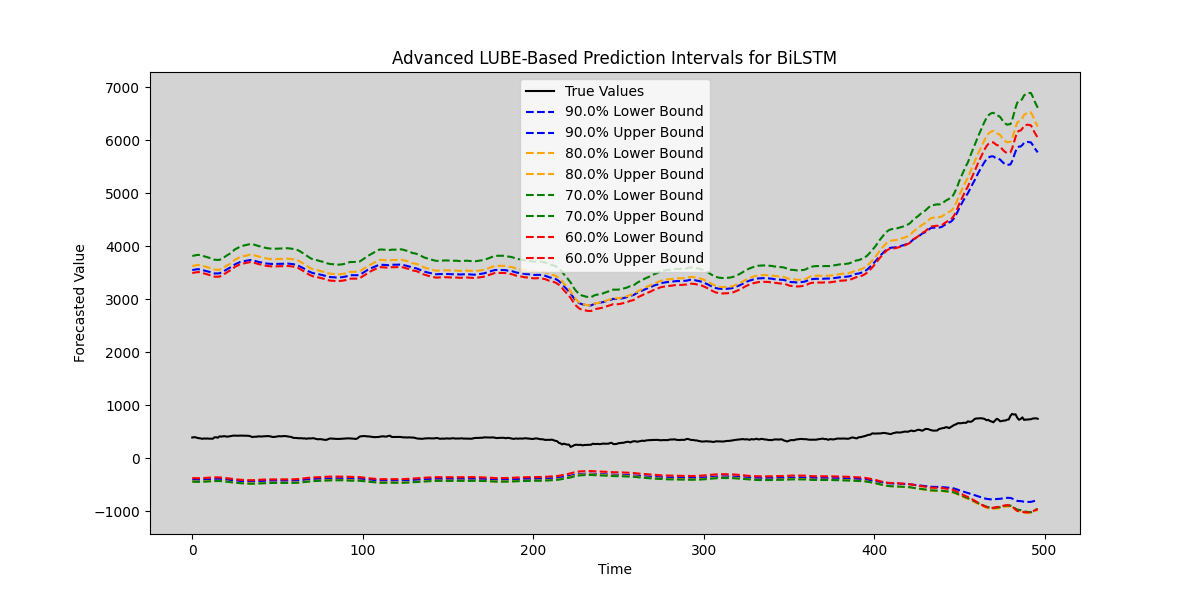
\includegraphics[width=\textwidth]{Chap02/figs/BiLSTM_advanced_lube_plot_ADANIPORTS.png}
                \caption{BiLSTM.}
            \end{subfigure}
            \hfill
            \begin{subfigure}[b]{\textwidth}
                \centering
                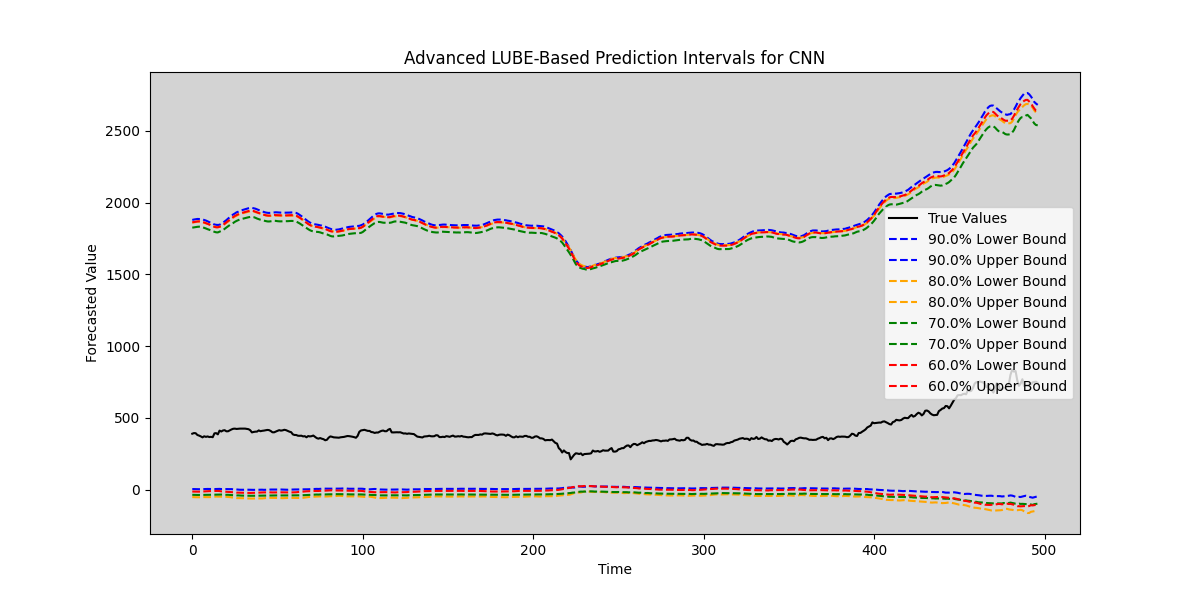
\includegraphics[width=\textwidth]{Chap02/figs/CNN_advanced_lube_plot_ADANIPORTS.png}
                \caption{CNN.}
            \end{subfigure}
            \begin{subfigure}[b]{\textwidth}
                \centering
                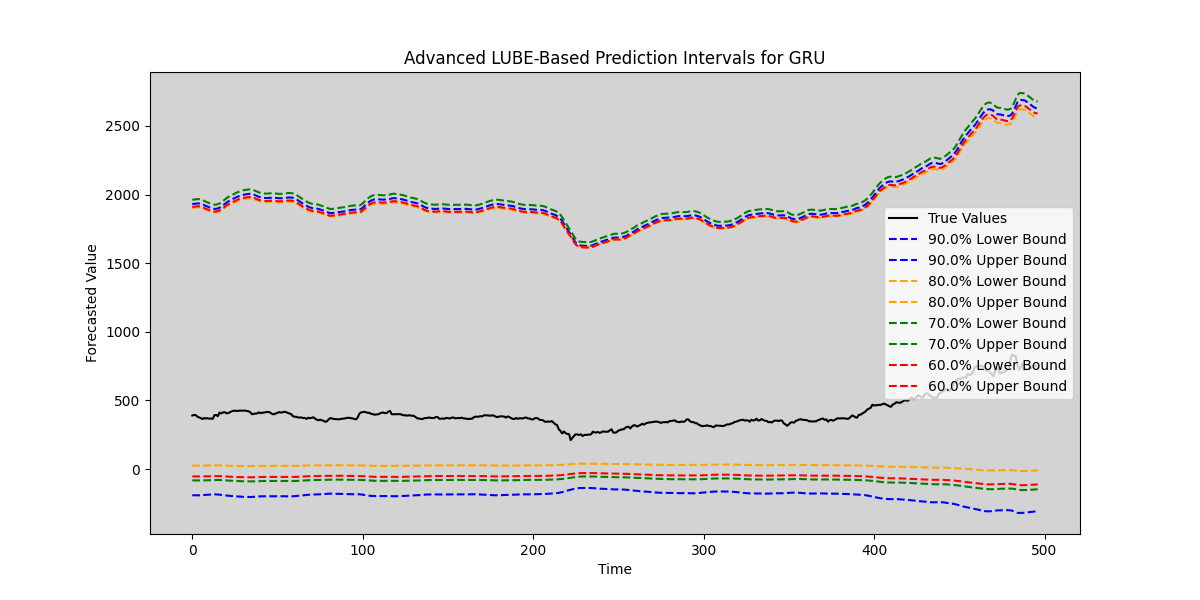
\includegraphics[width=\textwidth]{Chap02/figs/GRU_advanced_lube_plot_ADANIPORTS.png}
                \caption{GRU.}
            \end{subfigure}
            \begin{subfigure}[b]{\textwidth}
                \centering
                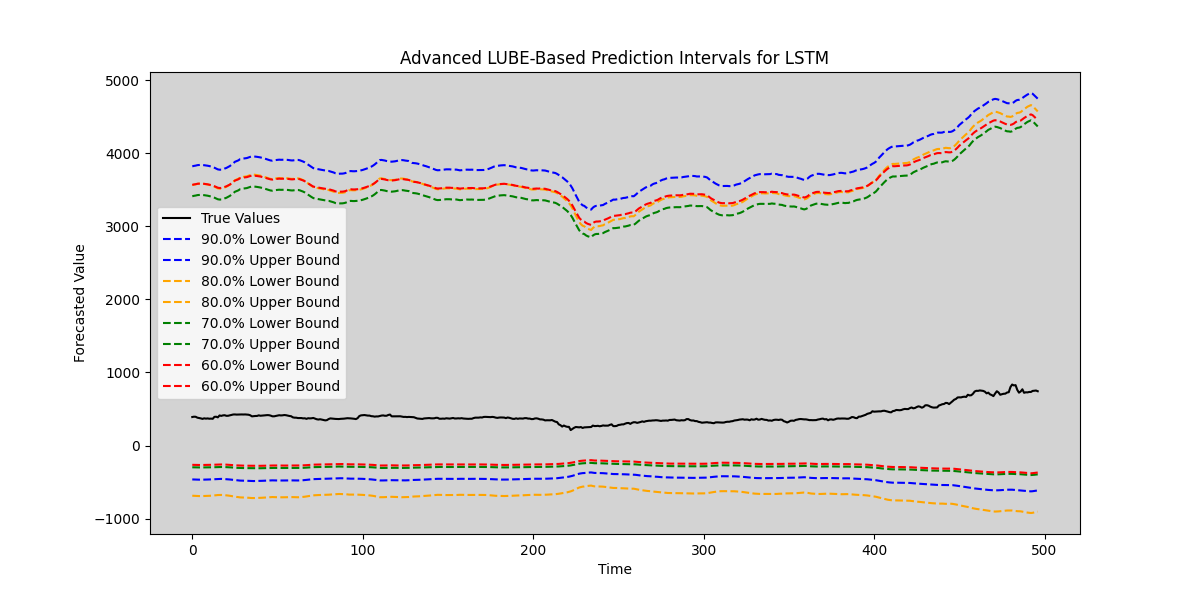
\includegraphics[width=\textwidth]{Chap02/figs/LSTM_advanced_lube_plot_ADANIPORTS.png}
                \caption{LSTM.}
            \end{subfigure}
        \end{minipage}
    
    \caption{Prediction Intervals for Adani Ports dataset obtained using Advanced LUBE method and (a) BiLSTM, (b) CNN, (c) GRU, (d) LSTM Models.}
    \label{Fi 3.2}
\end{figure}

Probabilistic forecasting methodologies have been tested on five disparate datasets: Adani Ports, Asian Paints, Axis Bank, Electricity Consumption Load, and Web Traffic. The six methodologies like Traditional LUBE, Advanced LUBE, QR-based, Bootstrap-based, Gaussian Distribution, and Weibull Distribution were used in all cases of these analyses. The performance was evaluated using the four critical metrics, which included Prediction Interval Coverage Probability (PICP), Prediction Interval Normalized Average Width (PINAW), Average Coverage Error (ACE), and Average Width Error (AWE). The following is a more detailed summary of the results and insights learned from the analysis of all five datasets:

\subsection{Performance Of Each Method Across Datasets}
The Traditional LUBE approach consistently achieved near-optimal PICP across all confidence levels and datasets, demonstrating reliable interval coverage. However, it generally produced wider prediction intervals, reflected in higher PINAW values—for instance, a PINAW of 10.01 at the 90\% confidence level with CNN DL model for the Adani Ports dataset \ref{Table 1}, indicating a highly conservative prediction. Similar trends were observed in the Asian Paints dataset, where the LSTM model showed a PINAW of 5.87 at 90\% confidence level. \ref{Table 2} Furthermore, across all datasets, the Traditional LUBE method exhibited higher AWE values compared to other methods, pointing to less efficient interval calibration. This trade-off suggests that while Traditional LUBE is dependable, it tends to produce overly cautious intervals, particularly in models like BiLSTM. In contrast, the Advanced LUBE method demonstrated superior performance across all datasets by generating narrower yet highly covered intervals. For example, in the Electricity Consumption dataset \ref{Table 4}, the GRU model achieved a PICP of 100\% with a significantly narrower PINAW of 1.35 at 90\% confidence level when compared to Traditional LUBE's 2.25. Similarly, in the Web Traffic dataset \ref{Table 5}, CNN attained a PINAW of 1.69 with a PICP of 99.19\% at 90\% confidence level. Additionally, the Advanced LUBE method consistently yielded lower ACE and AWE values, confirming its capability to deliver more dependable and efficient prediction intervals. The QR-based method, while producing the narrowest intervals among non-parametric approaches, often suffered from under-coverage. For instance, in the Axis Bank dataset at the 90\% confidence level, the BiLSTM model reached 96.65\% PICP with a very low PINAW of 0.15 \ref{Table 3}. Thus, despite its precision, the QR-based method falls short in applications requiring high reliability. The Bootstrap-based method held an intermediate location on interval coverage and width, with competitive PINAW and PICP values but not entirely on par with consistency of LUBE or Advanced LUBE. On the Adani Ports dataset, for example, the GRU model had a PICP of 68.43\% supported by a PINAW of 0.28 at 70\% confidence level which is a desirable output, while on the Electricity Consumption dataset, the GRU model held a PICP of only 28.20\% supported by a PINAW of 0.10 at 70\% confidence level \ref{Table 4} which is not at all desirable and shows major undercoverage. The Gaussian distribution method consistently produced the most narrow intervals but often failed to achieve the targeted PICP thresholds. On the Asian Paints dataset, for example, it had a PINAW of 0.42 at confidence level 70\% but a PICP of 83.58\%, supported by high ACE value of 13.58 indicating under coverage \ref{Table 6}. On the other hand, the Weibull distribution showed better PICP performance than Gaussian at 92.90\% at 90\% confidence on the Web Traffic dataset but at the cost of wider intervals (PINAW = 0.76) \ref{Table 10}.  Even though Weibull had better reliability, its relatively higher AWE values compared to Gaussian indicated lower efficiency and hence was better suited for application where coverage takes precedence over narrow intervals. Advanced LUBE hence proved to be the best overall and reliable methodology with high efficiency and reliability on a range of datasets and models. The Gaussian and Weibull Distribution Tables are shown in Tables \ref{Table 6} to \ref{Table 10}.

\subsection{Dataset Specific Observations}
The stock prices data for Adani Ports, Asian Paints and Axis Bank indicated consistent trends, with both the Traditional and Advanced LUBE methods indicating high PICP values. Fig \ref{Fi 3.2}, Fig. \ref{Fi 3.3} Significant differences, however, were observed among the widths of the intervals, with the Advanced LUBE technique showing a tendency to generate more tightened intervals. The QR-based and Bootstrap methods generated more efficient (narrow) intervals;Fig. \ref{Fi 3.3} Fig. \ref{Fi 3.4} however, these came at the cost of reliability as the coverage levels were lower. The data for Electricity Consumption Load indicated the applicability and efficiency of the Advanced LUBE methodology, which obtained high coverage along with efficient interval lengths, while the QR-based and Bootstrap methods indicated poor performance with very low PICP values. A similar trend was also observed for the Web Traffic dataset, where both the Advanced LUBE and Bootstrap methods indicated relatively higher effectiveness by balancing coverage and interval widths.

\subsection{Recommendations}
The Advanced LUBE method is best suited for applications that demand high reliability alongside efficient interval widths as it consistently outperformed other approaches across all datasets and evaluation metrics. The Bootstrap-based method serves well in scenarios where a moderate level of reliability is acceptable, offering a balanced trade-off between coverage and interval width. Among the parametric methods, the Gaussian approach yields very narrow and precise intervals but suffers from under-coverage, making it less reliable Fig. \ref{Fi 3.6}. In contrast, the Weibull distribution delivers better coverage but tends to produce wider intervals, reducing its efficiency for applications requiring tightly bound predictions Fig. \ref{Fi 3.7}.

\begin{figure}[H]
    \centering
        \begin{minipage}{0.6\textwidth}
            \centering
            \begin{subfigure}[b]{1.0\textwidth}
                \centering
                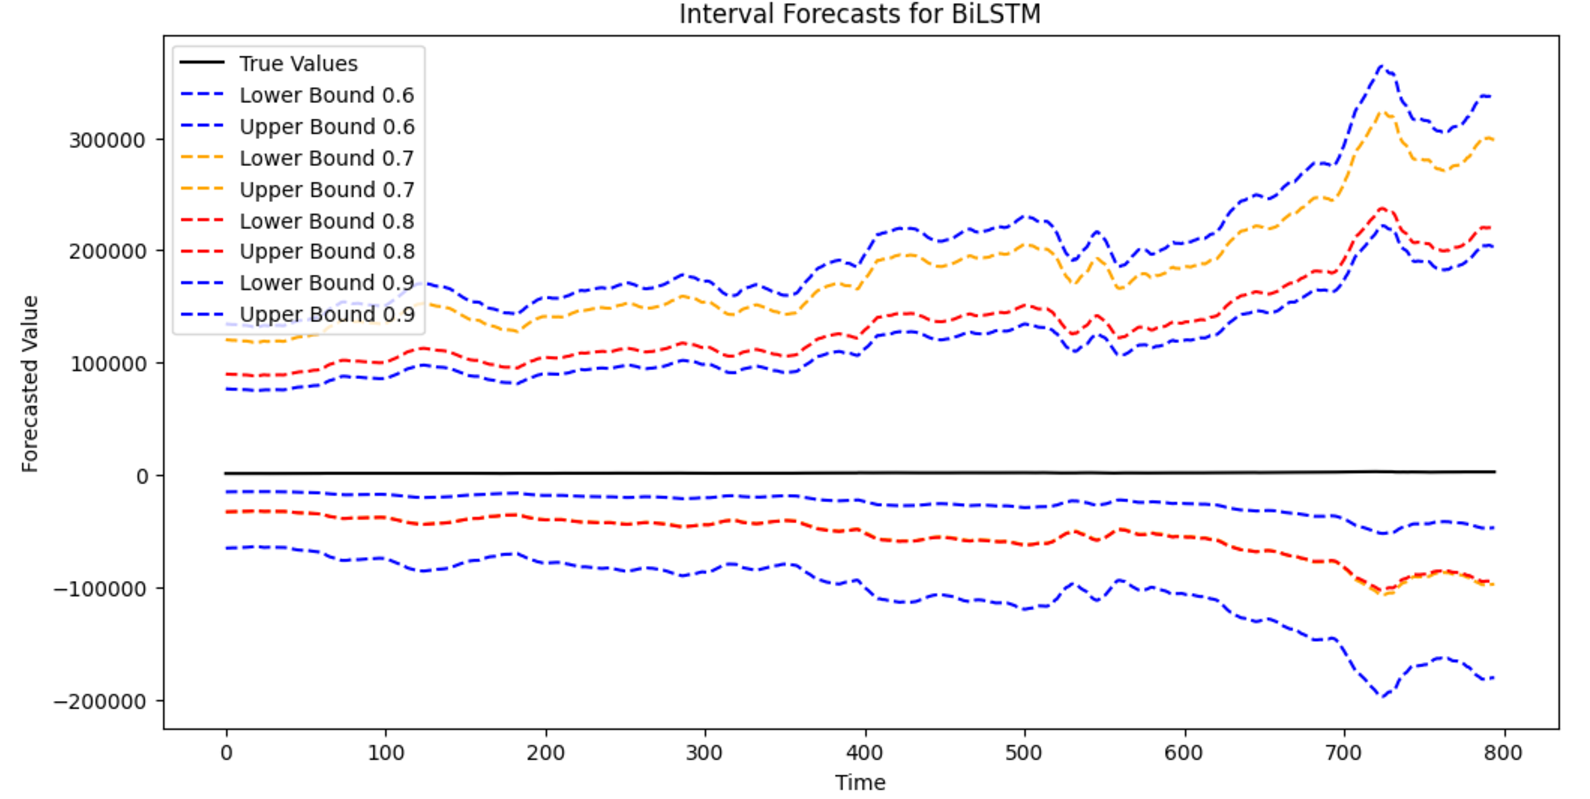
\includegraphics[width=\textwidth]{Chap02/figs/LUBE_BiLSTM_AsianPaints.png}
                \caption{BiLSTM.}
            \end{subfigure}
            \hfill
            \begin{subfigure}[b]{1.0\textwidth}
                \centering
                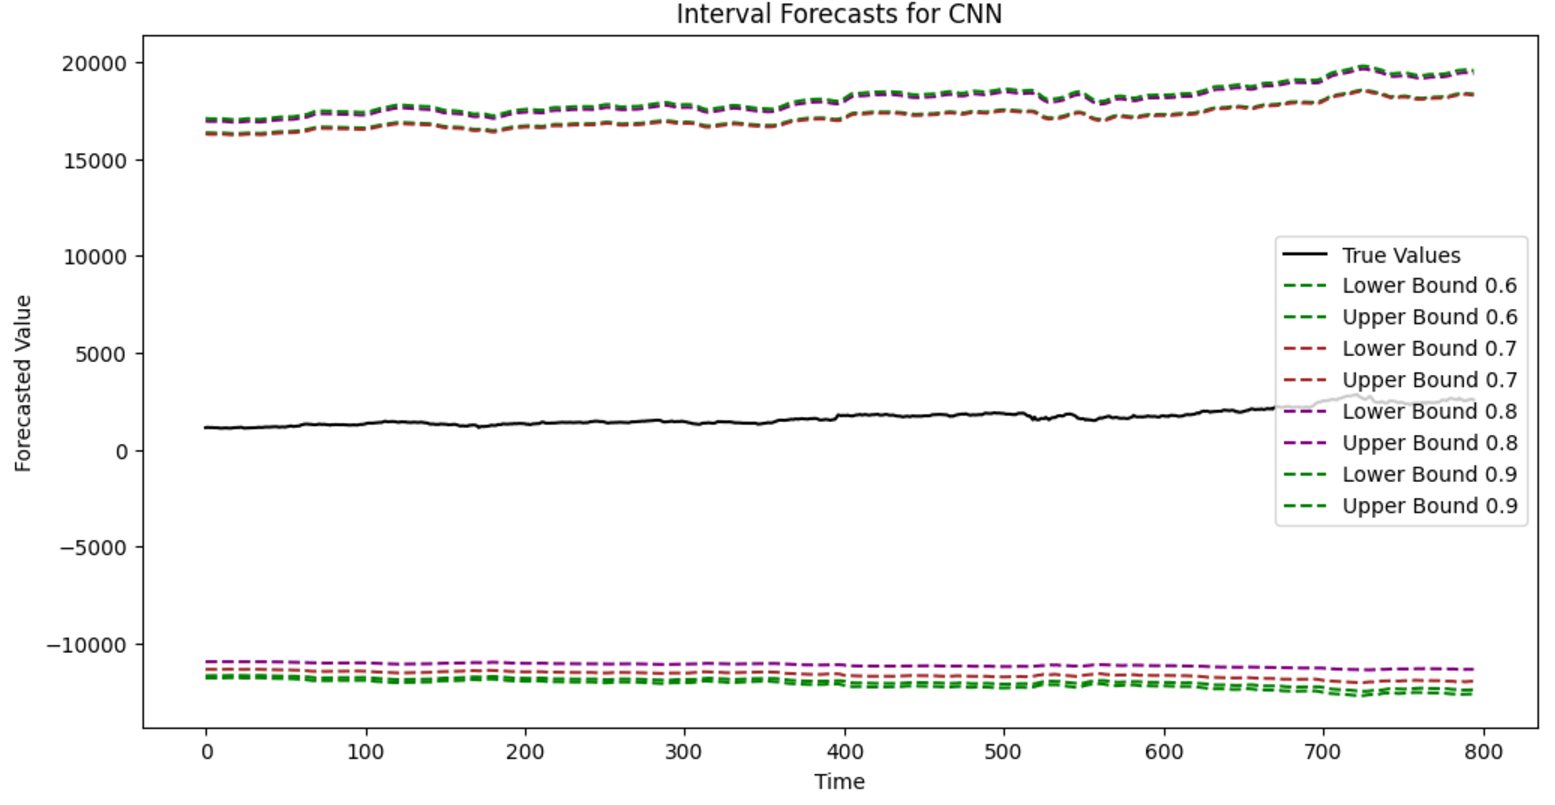
\includegraphics[width=\textwidth]{Chap02/figs/LUBE_CNN_AsianPaints.png}
                \caption{CNN.}
            \end{subfigure}
            \begin{subfigure}[b]{1.0\textwidth}
                \centering
                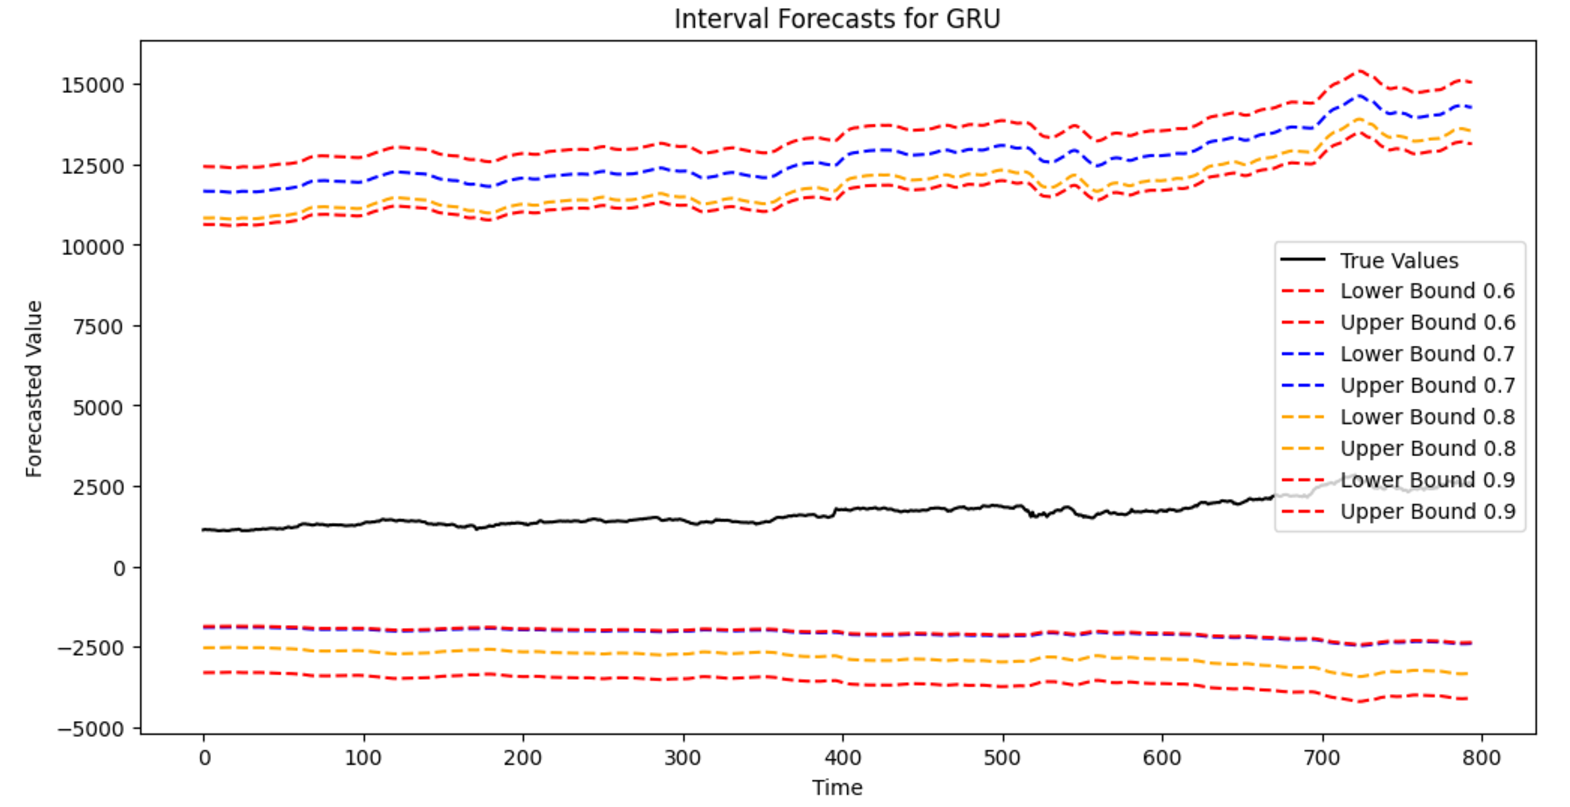
\includegraphics[width=\textwidth]{Chap02/figs/LUBE_GRU_AsianPaints.png}
                \caption{GRU.}
            \end{subfigure}
            \begin{subfigure}[b]{1.0\textwidth}
                \centering
                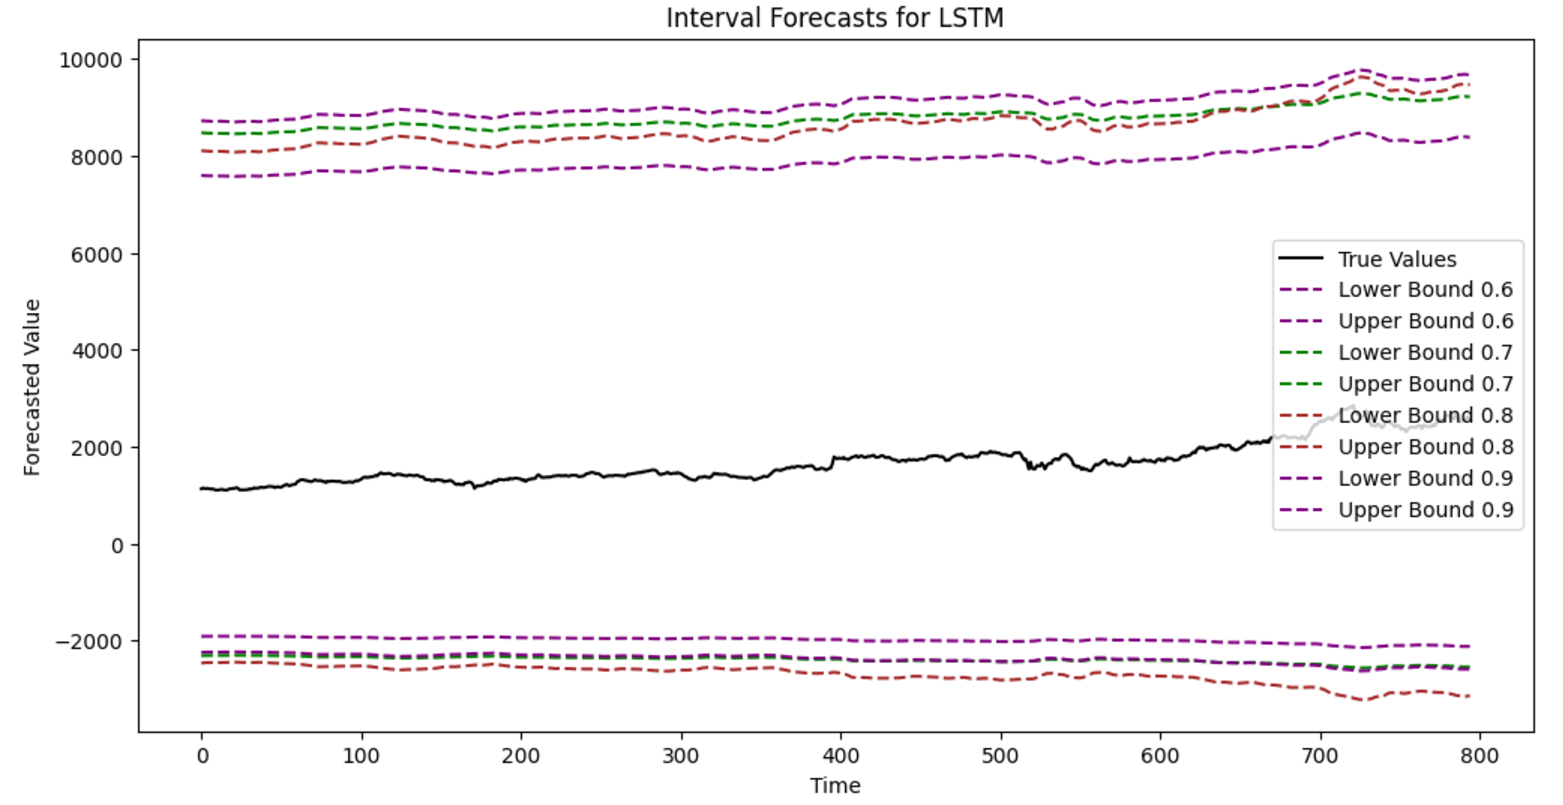
\includegraphics[width=\textwidth]{Chap02/figs/LUBE_LSTM_AsianPaints.png}
                \caption{LSTM.}
            \end{subfigure}
        \end{minipage}
    
    \caption{Prediction Intervals for Asian Paints dataset obtained using Traditional LUBE method and (a) BiLSTM, (b) CNN, (c) GRU, (d) LSTM Models.}
    \label{Fi 3.3}
\end{figure}

\begin{figure}[H]
    \centering
        \begin{minipage}{0.6\textwidth}
            \centering
            \begin{subfigure}[b]{1.0\textwidth}
                \centering
                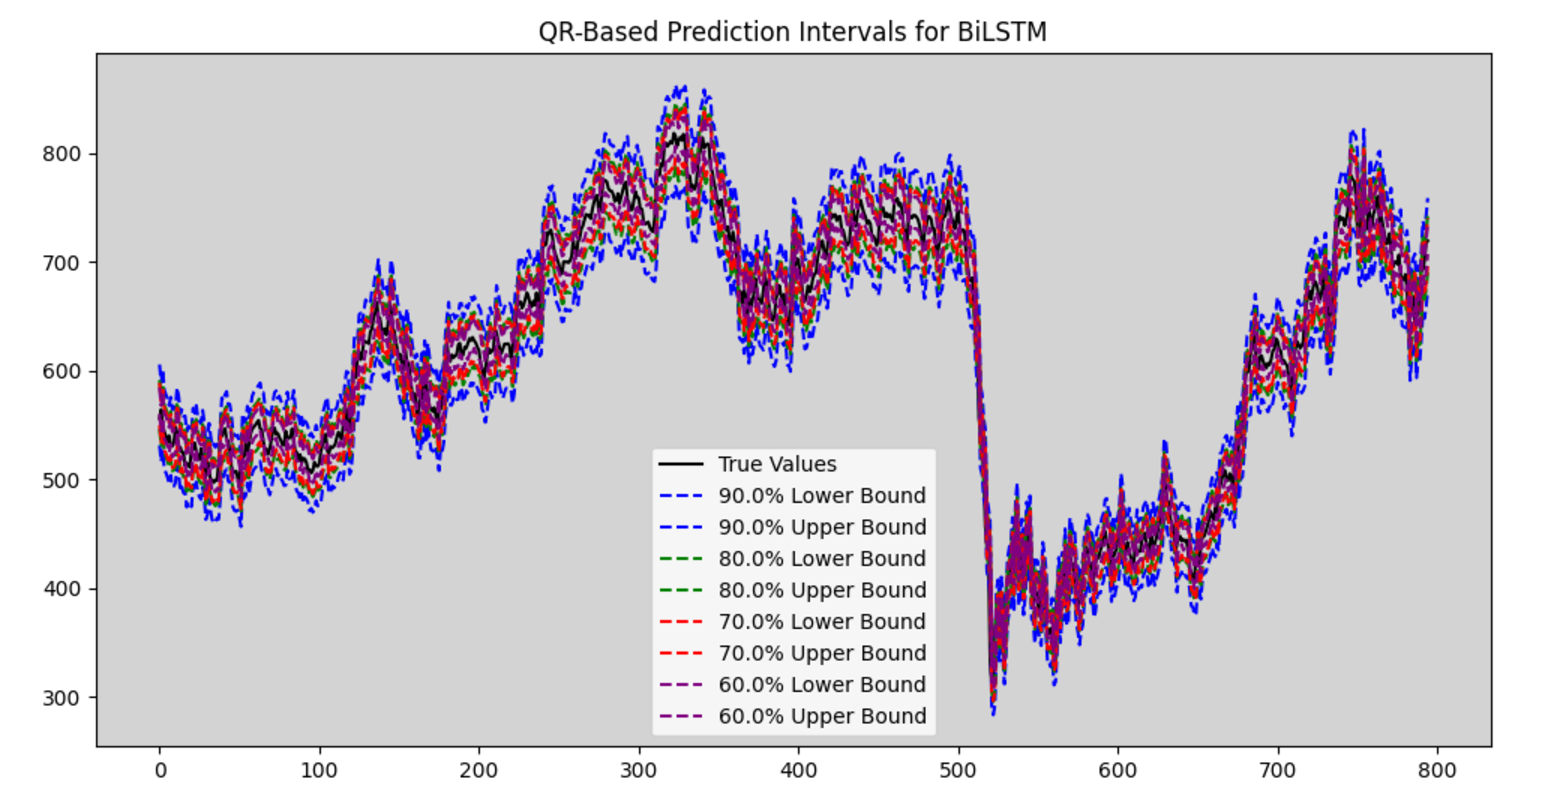
\includegraphics[width=\textwidth]{Chap02/figs/QR_BiLSTM_AxisBank_Original.png}
                \caption{BiLSTM.}
            \end{subfigure}
            \hfill
            \begin{subfigure}[b]{1.0\textwidth}
                \centering
                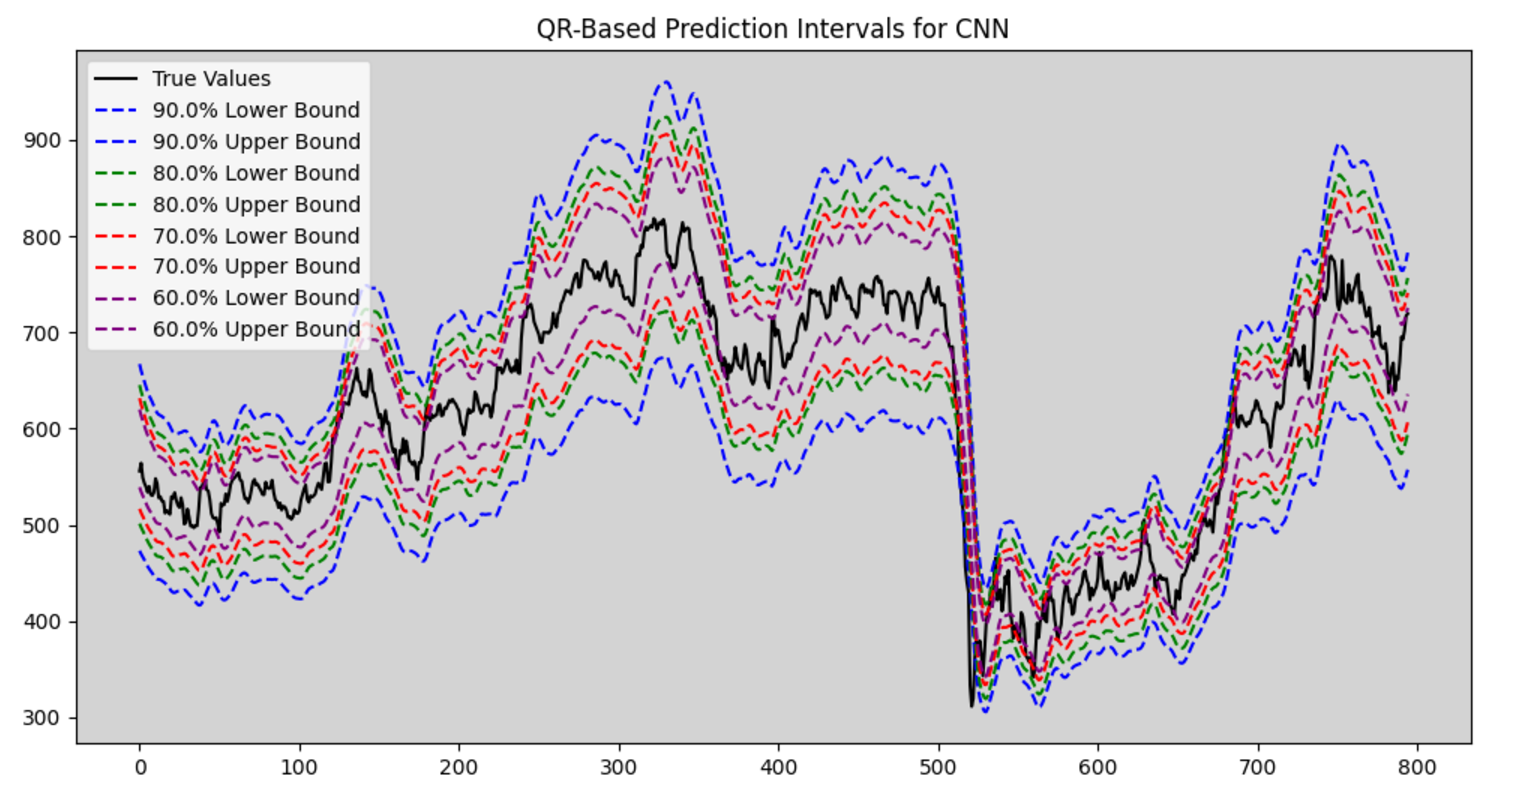
\includegraphics[width=\textwidth]{Chap02/figs/QR_CNN_AxisBank.png}
                \caption{CNN.}
            \end{subfigure}
            \begin{subfigure}[b]{1.0\textwidth}
                \centering
                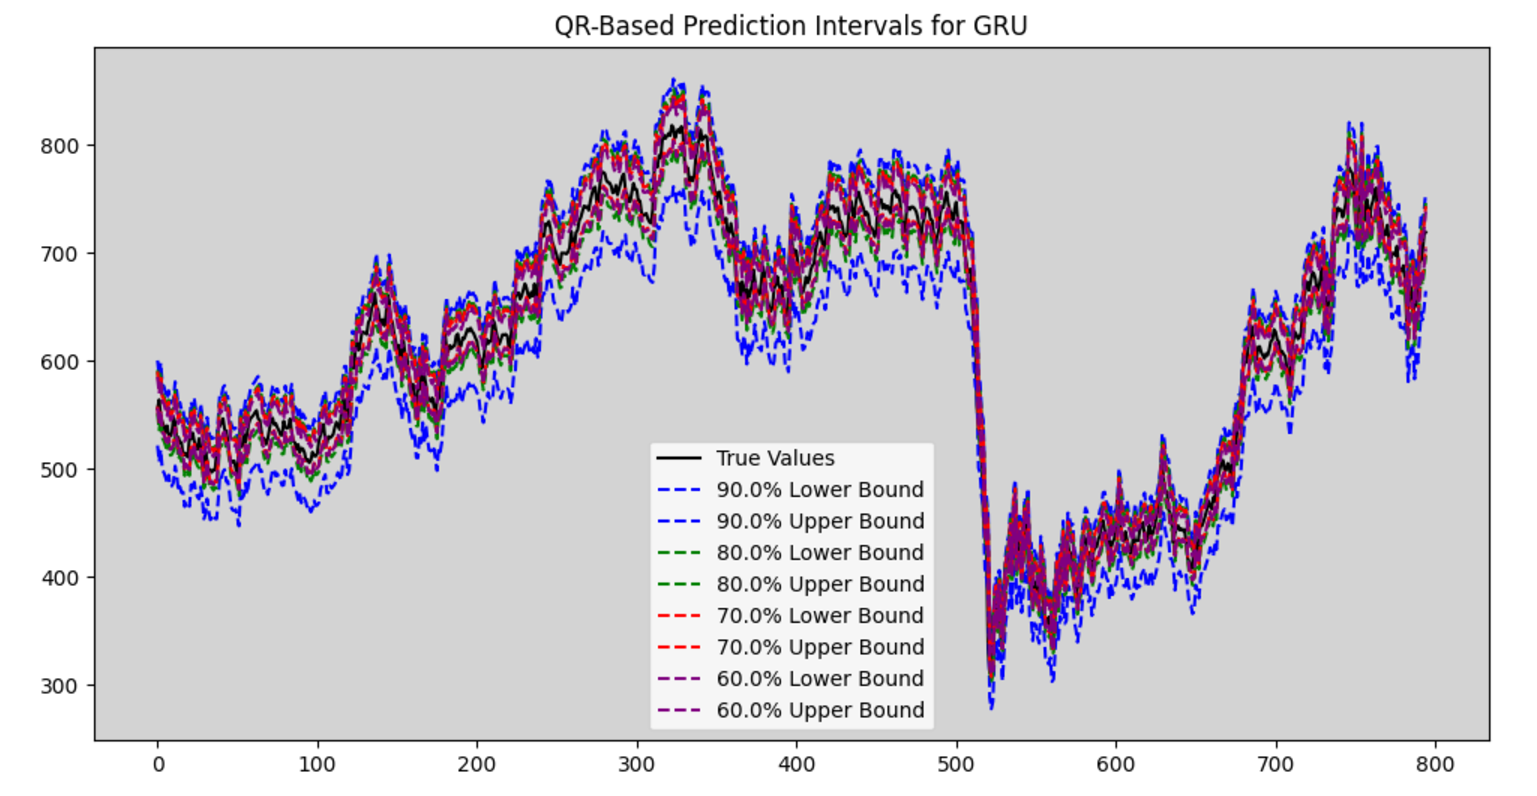
\includegraphics[width=\textwidth]{Chap02/figs/QR_GRU_AxisBank.png}
                \caption{GRU.}
            \end{subfigure}
            \begin{subfigure}[b]{1.0\textwidth}
                \centering
                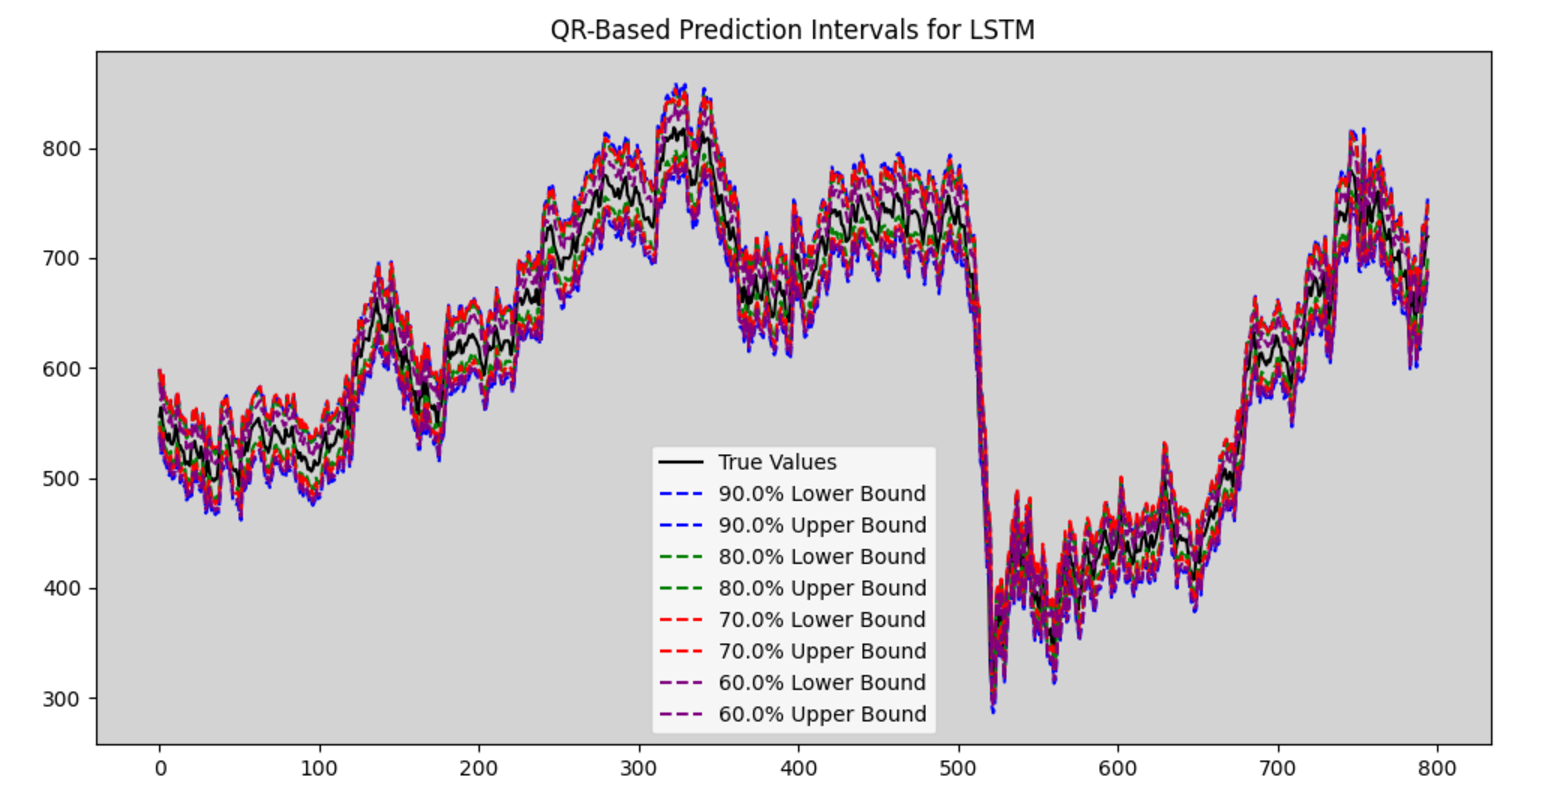
\includegraphics[width=\textwidth]{Chap02/figs/QR_LSTM_AxisBank.png}
                \caption{LSTM.}
            \end{subfigure}
        \end{minipage}
    
    \caption{Prediction Intervals for Axis Bank dataset obtained using QR-based method and (a) BiLSTM, (b) CNN, (c) GRU, (d) LSTM Models.}
    \label{Fi 3.4}
\end{figure}

\begin{figure}[H]
    \centering
        \begin{minipage}{0.6\textwidth}
            \centering
            \begin{subfigure}[b]{1.0\textwidth}
                \centering
                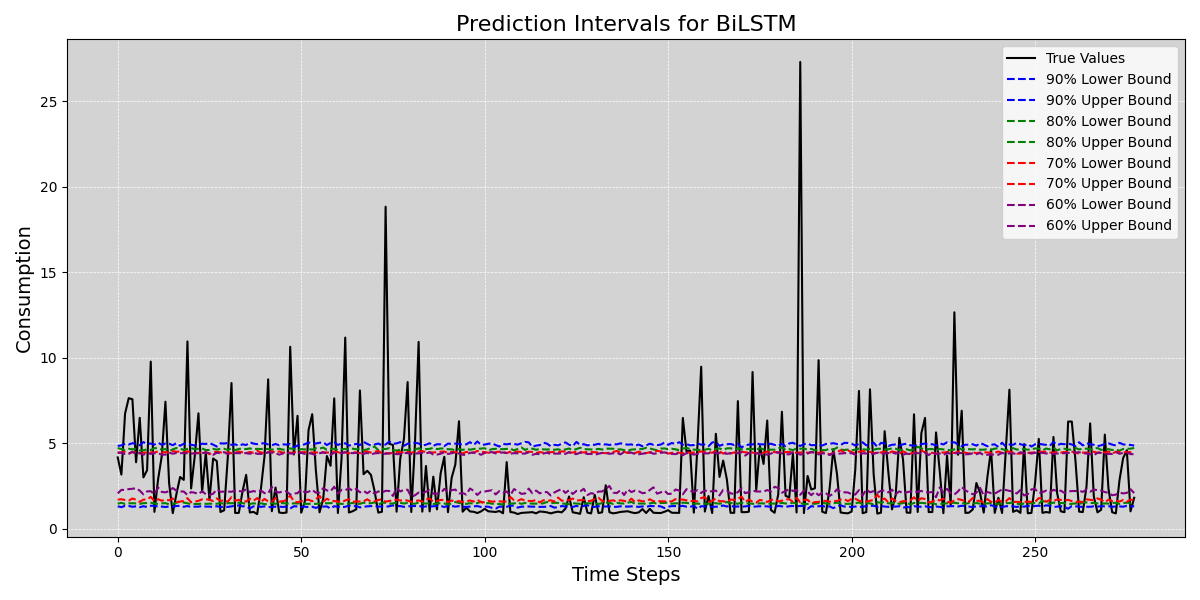
\includegraphics[width=\textwidth]{Chap02/figs/Prediction_Intervals_Styled_BiLSTM_Electricity_Consumption.png}
                \caption{BiLSTM.}
            \end{subfigure}
            \hfill
            \begin{subfigure}[b]{1.0\textwidth}
                \centering
                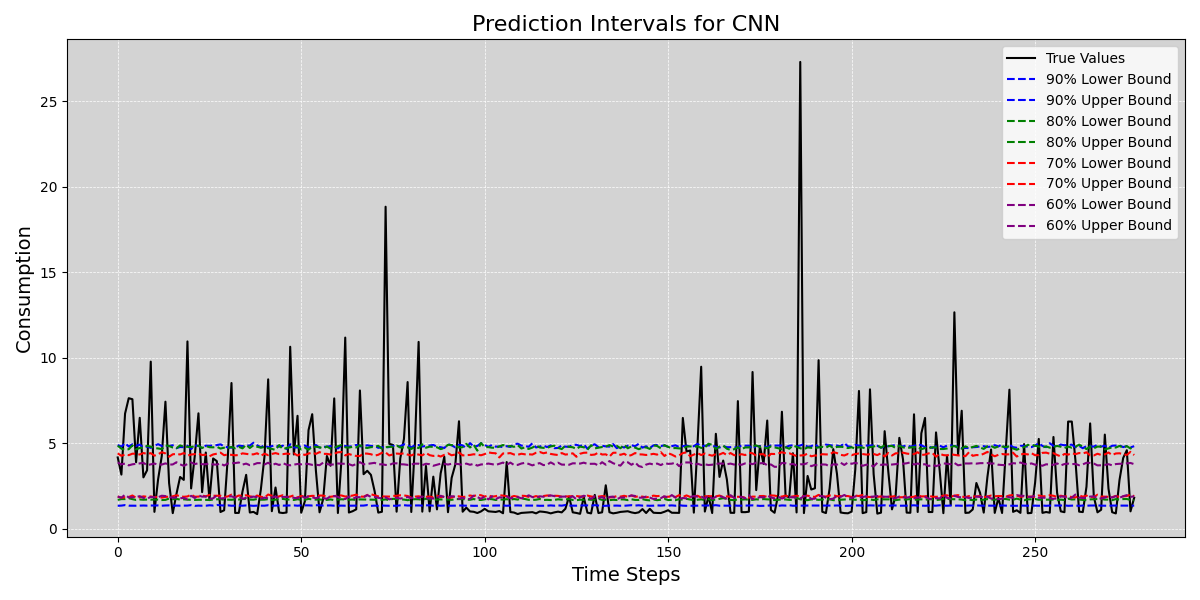
\includegraphics[width=\textwidth]{Chap02/figs/Prediction_Intervals_Styled_CNN_Electricity_Consumption.png}
                \caption{CNN.}
            \end{subfigure}
            \begin{subfigure}[b]{1.0\textwidth}
                \centering
                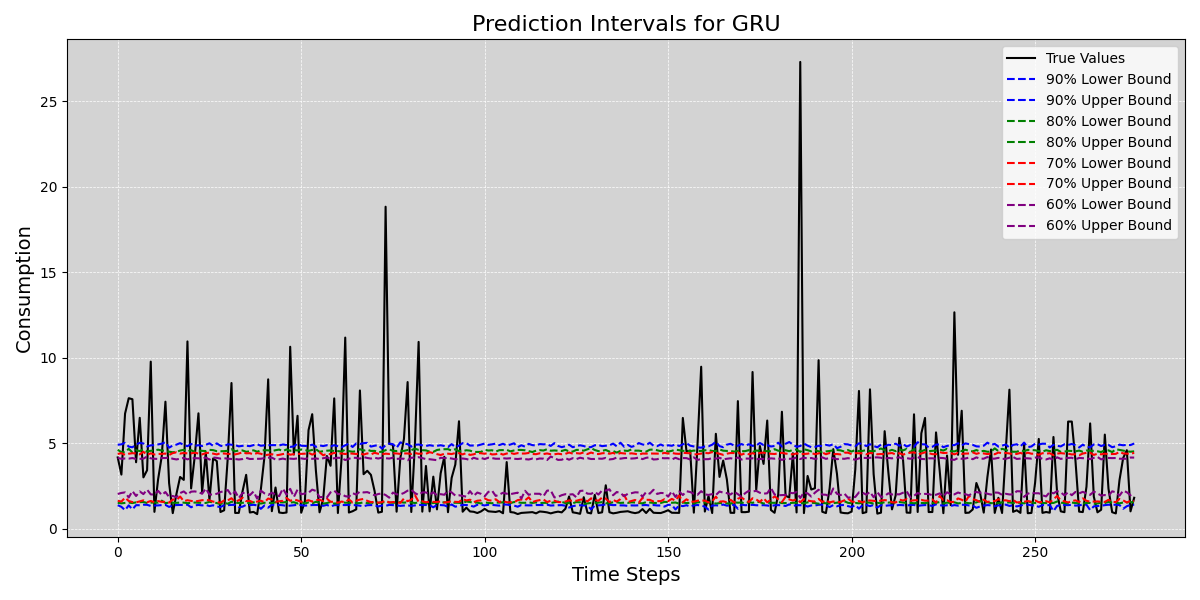
\includegraphics[width=\textwidth]{Chap02/figs/Prediction_Intervals_Styled_GRU_Electricity_Consumption.png}
                \caption{GRU.}
            \end{subfigure}
            \begin{subfigure}[b]{1.0\textwidth}
                \centering
                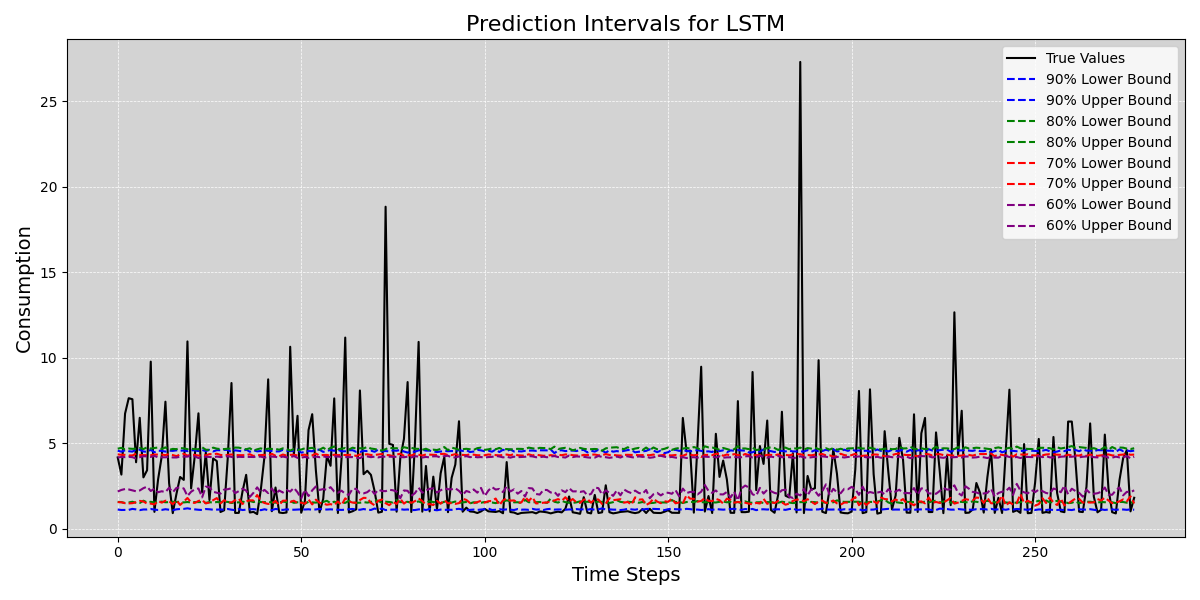
\includegraphics[width=\textwidth]{Chap02/figs/Prediction_Intervals_Styled_LSTM_Electricity_Consumption.png}
                \caption{LSTM.}
            \end{subfigure}
        \end{minipage}
    
    \caption{Prediction Intervals for Electricity Consumption dataset obtained using Bootstrap-based method and (a) BiLSTM, (b) CNN, (c) GRU, (d) LSTM Models.}
    \label{Fi 3.5}
\end{figure}

\begin{figure}[H]
    \centering
        \begin{minipage}{0.6\textwidth}
            \centering
            \begin{subfigure}[b]{0.8\textwidth}
                \centering
                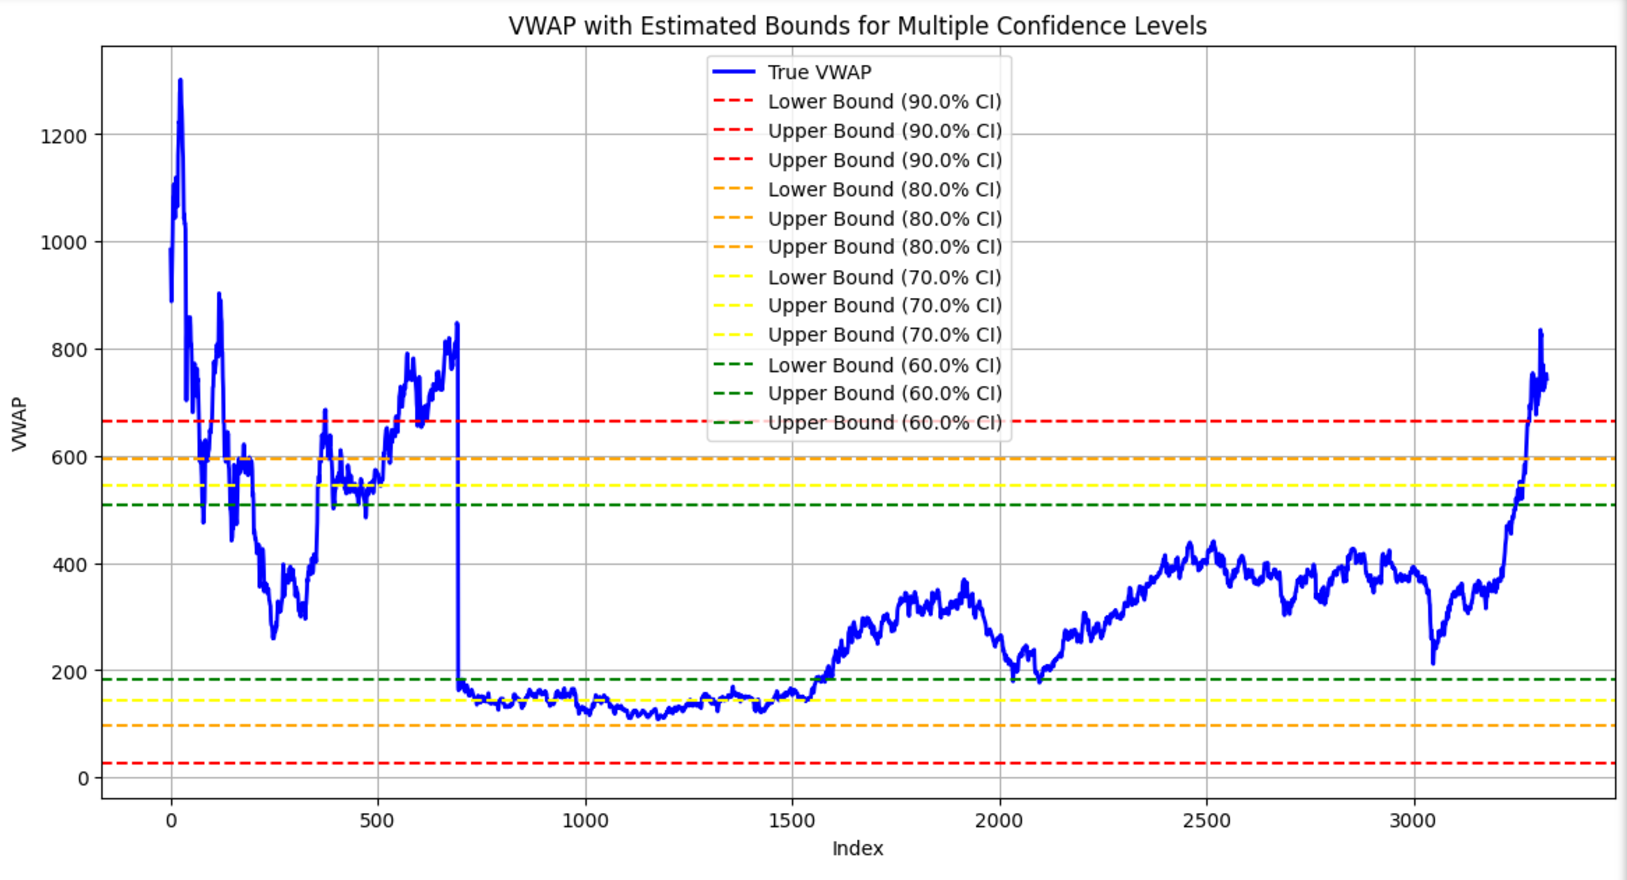
\includegraphics[width=\textwidth]{Chap02/figs/Gaussian_AdaniPorts.png}
                \caption{Adani Ports Dataset.}
            \end{subfigure}
            \hfill
            \begin{subfigure}[b]{0.8\textwidth}
                \centering
                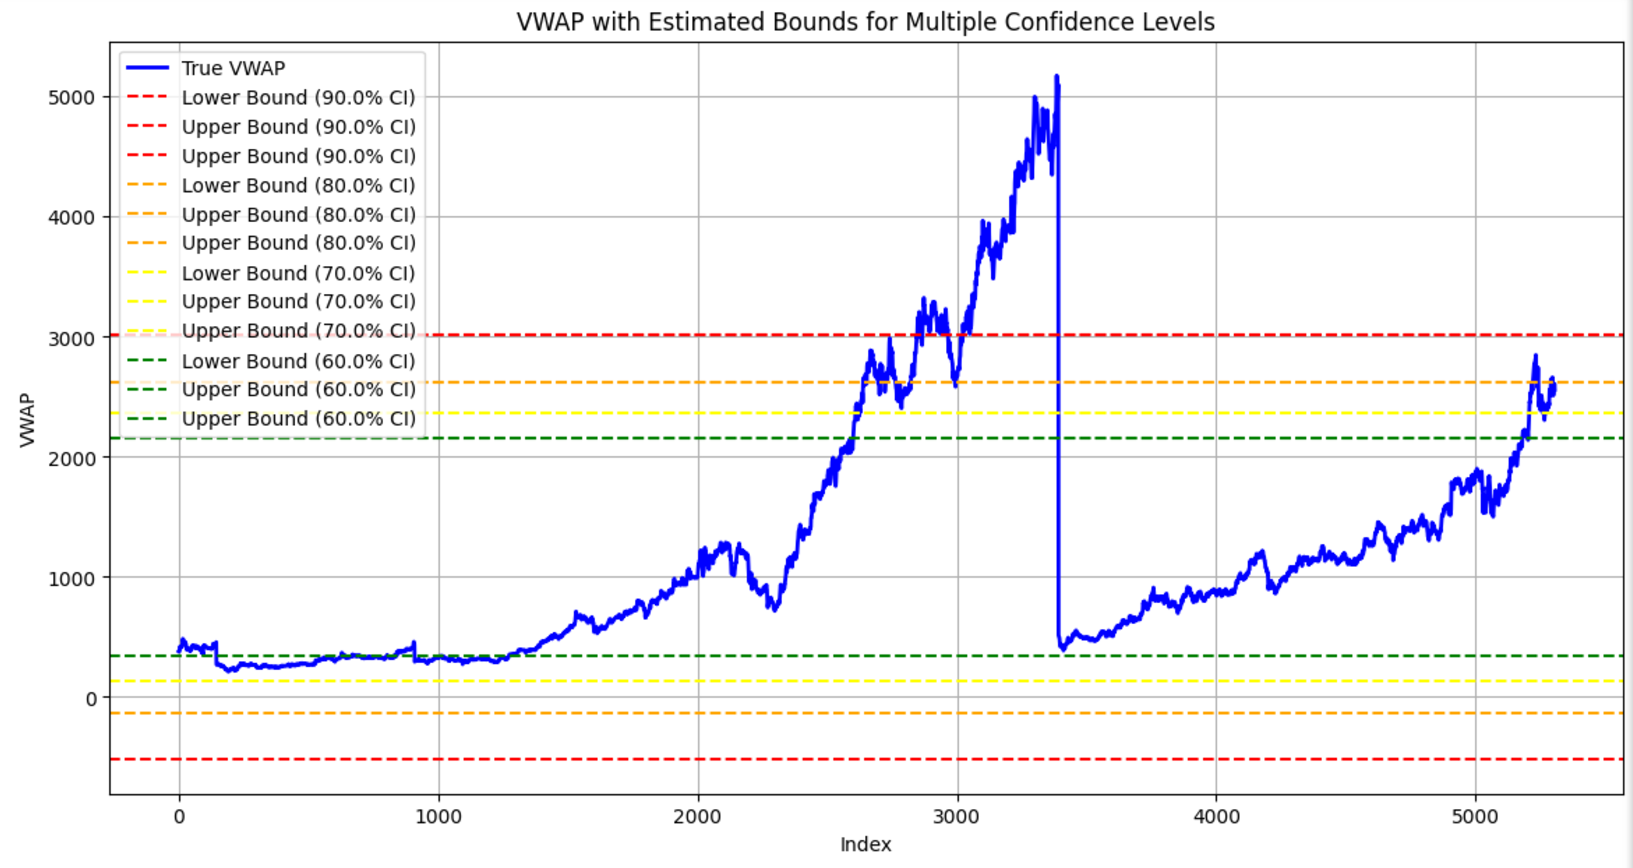
\includegraphics[width=\textwidth]{Chap02/figs/Gaussian_AsianPaints.png}
                \caption{Asian Paints Dataset.}
            \end{subfigure}
            \begin{subfigure}[b]{0.8\textwidth}
                \centering
                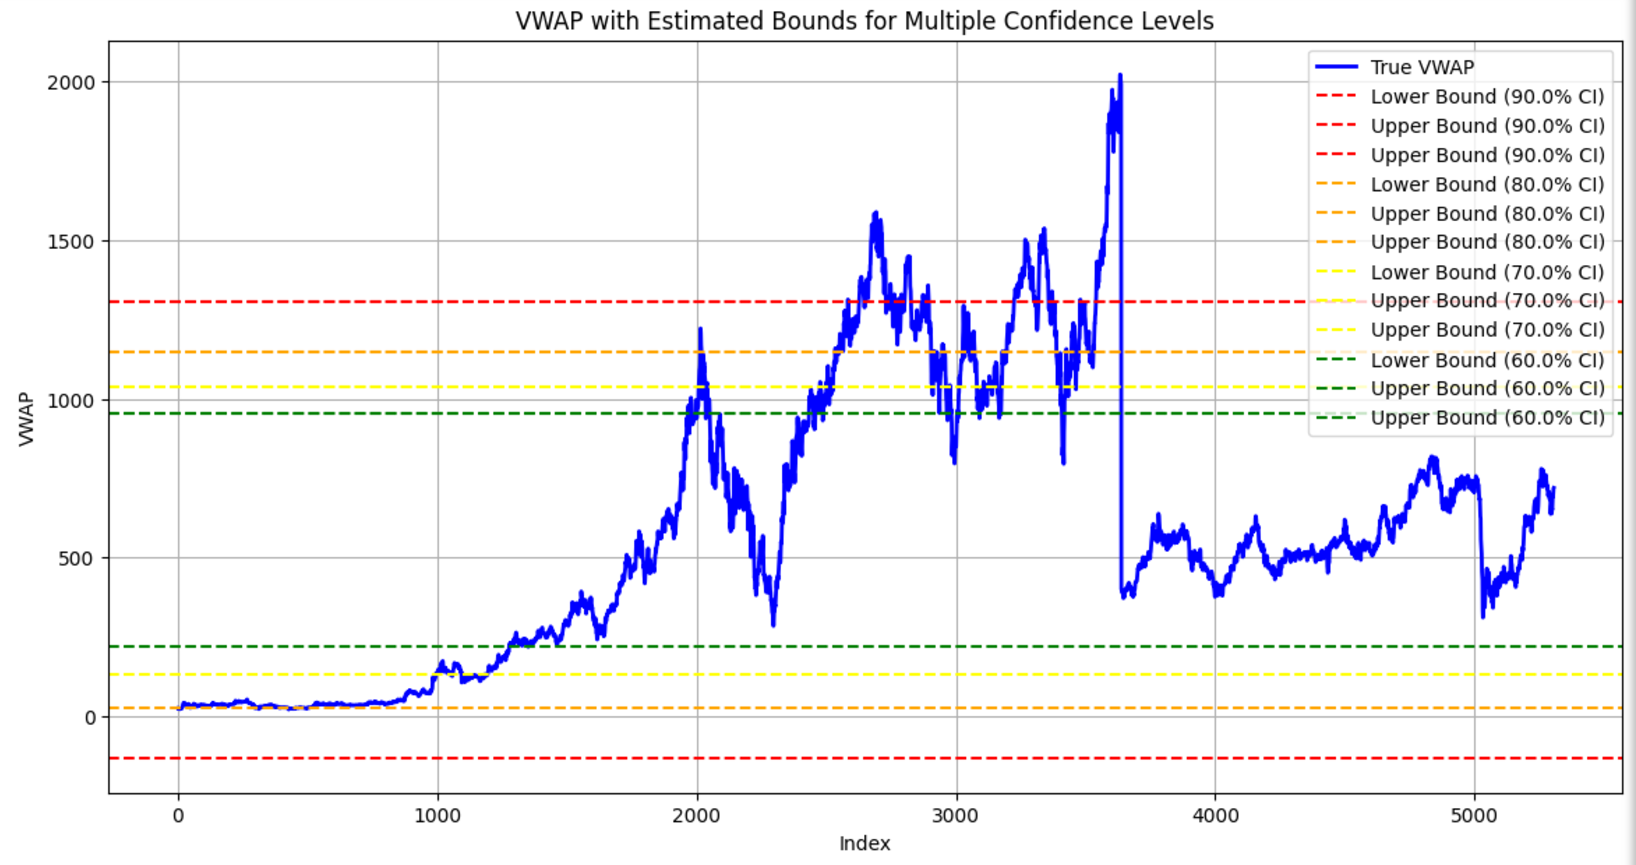
\includegraphics[width=\textwidth]{Chap02/figs/Gaussian_AxisBank.png}
                \caption{Axis Bank Dataset.}
            \end{subfigure}
            \begin{subfigure}[b]{0.8\textwidth}
                \centering
                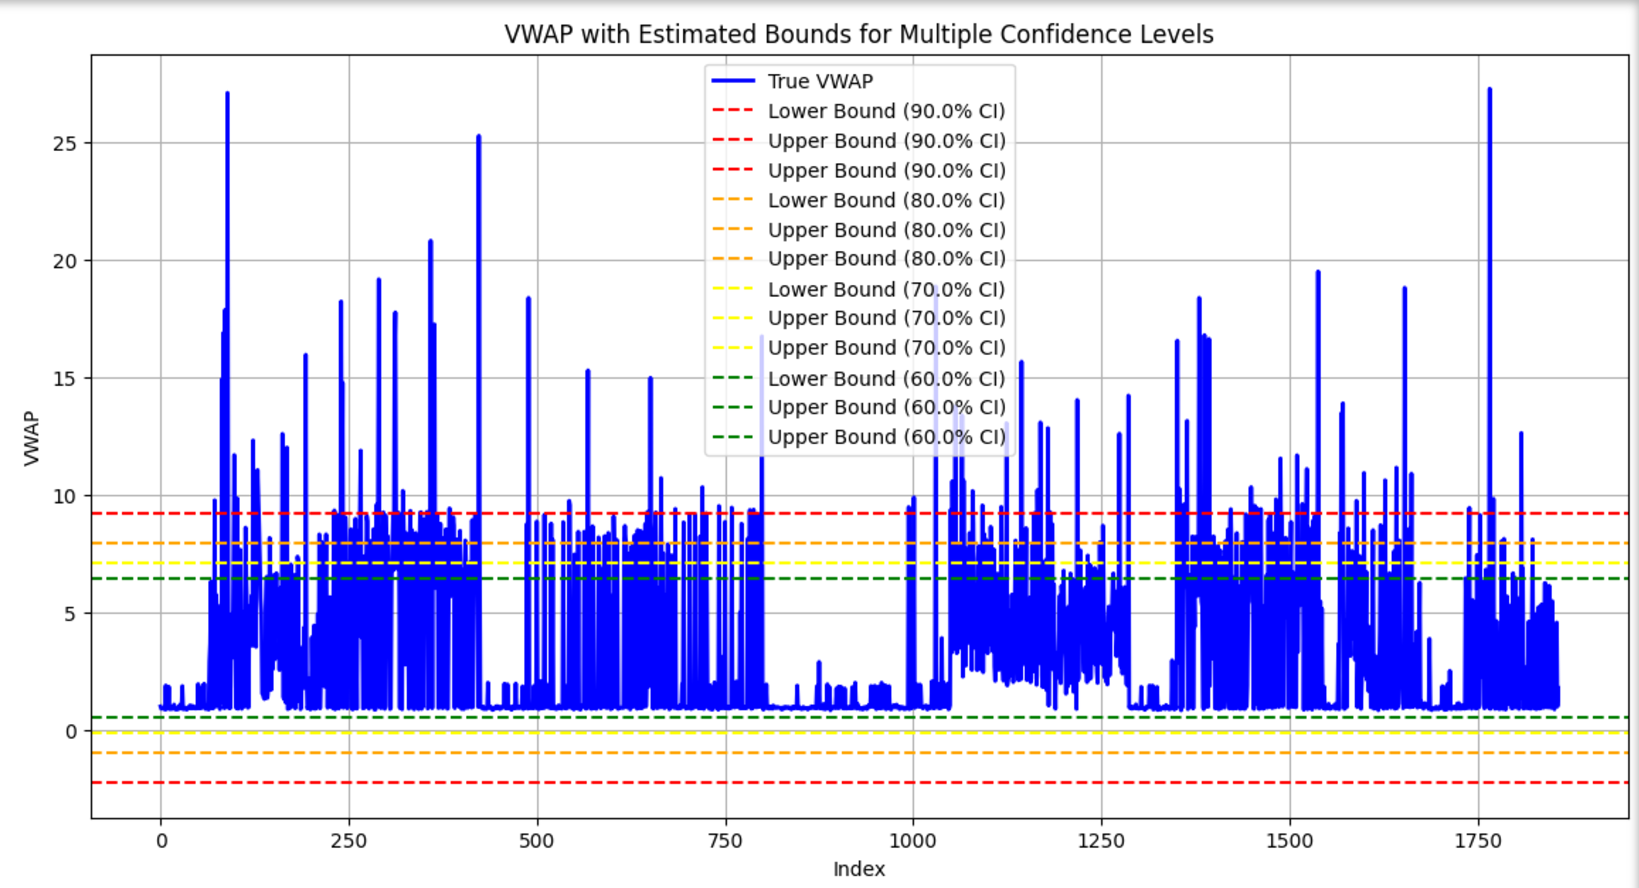
\includegraphics[width=\textwidth]{Chap02/figs/Gaussian_Electricity_Consumption.png}
                \caption{Electricity Consumption Dataset.}
            \end{subfigure}

            \begin{subfigure}[b]{0.8\textwidth}
                \centering
                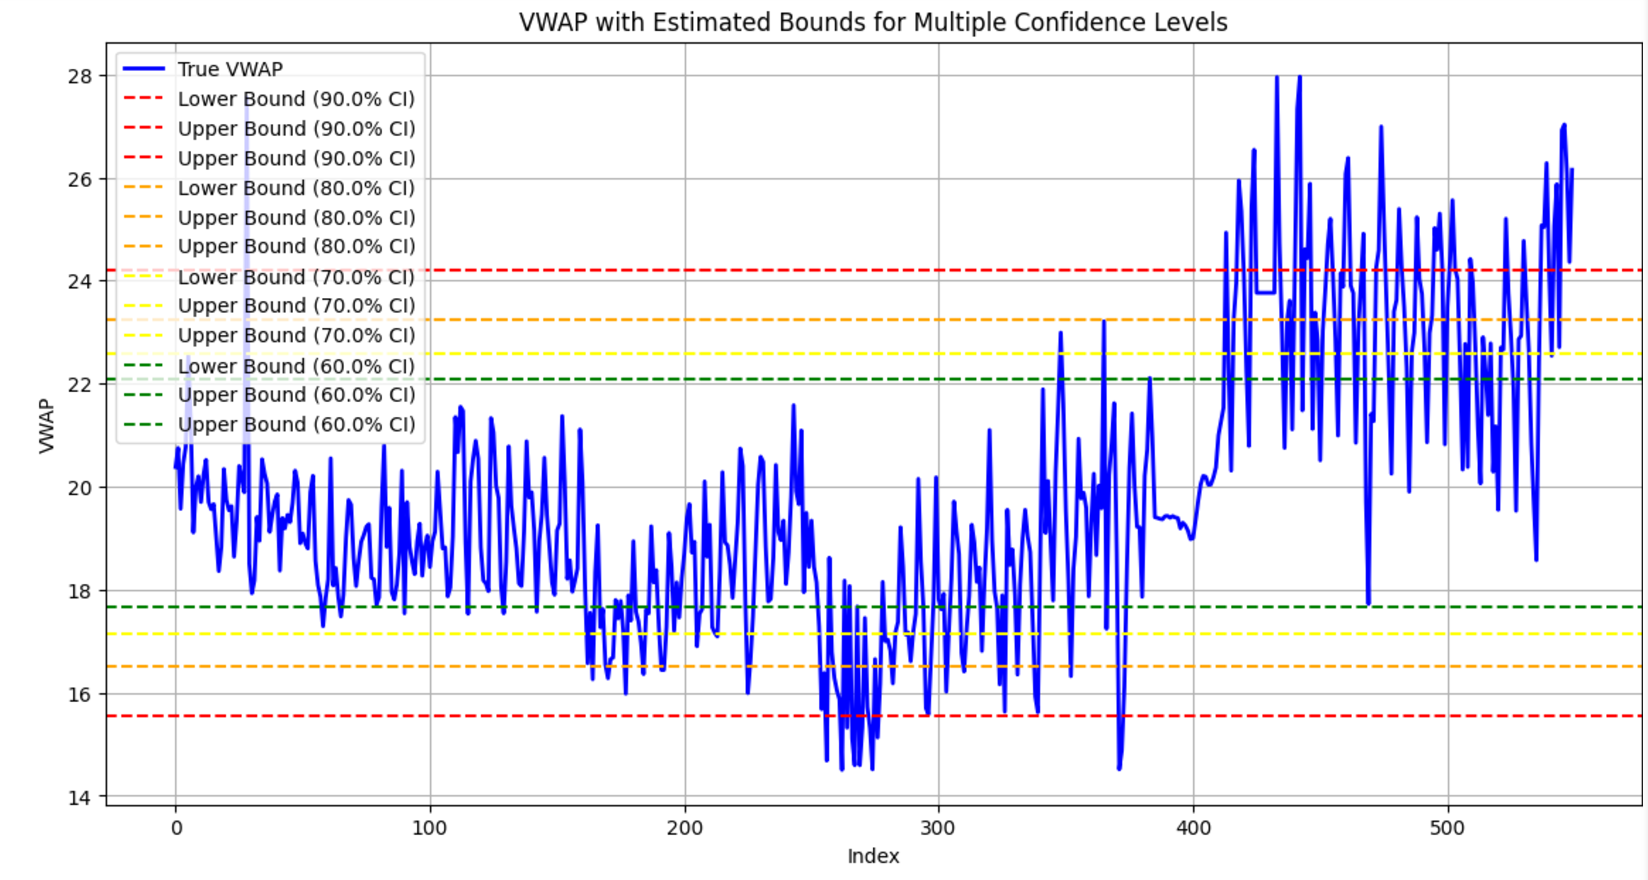
\includegraphics[width=\textwidth]{Chap02/figs/Gaussian_Web_Traffic.png}
                \caption{Web Traffic Dataset.}
            \end{subfigure}
        \end{minipage}
    
    \caption{Prediction Intervals for (a) Adani Ports, (b) Asian Paints, (c) Axis Bank, (d) Electricity Consumption Load, (e) Web Traffic datasets obtained using Gaussian Distribution method.}
    \label{Fi 3.6}
\end{figure}

\begin{figure}[H]
    \centering
        \begin{minipage}{0.6\textwidth}
            \centering
            \begin{subfigure}[b]{0.8\textwidth}
                \centering
                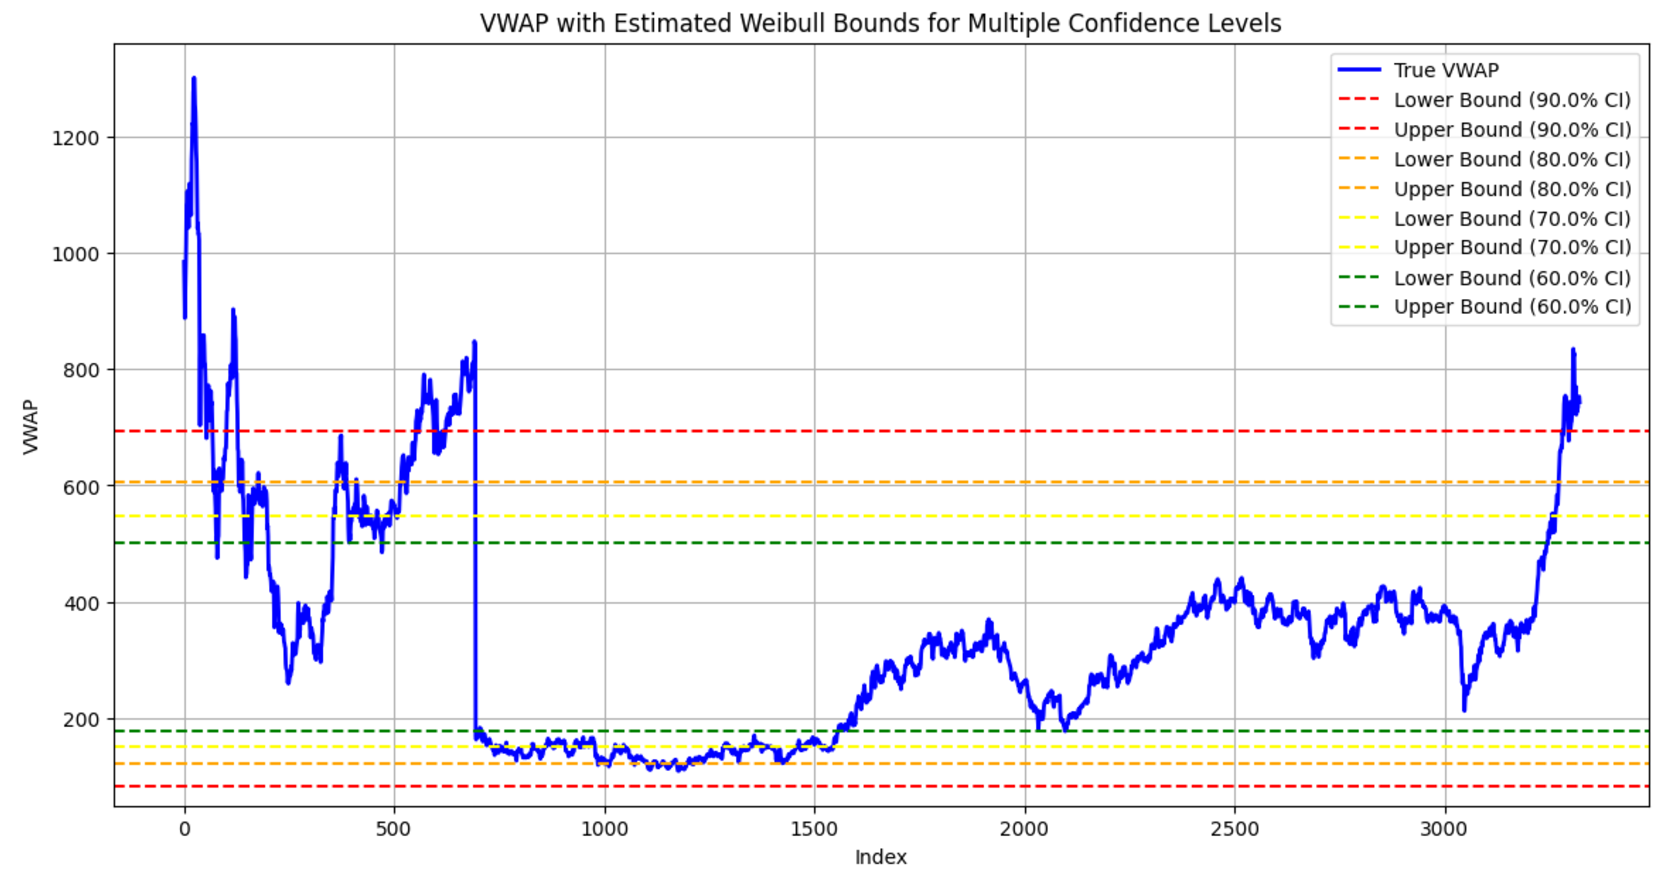
\includegraphics[width=\textwidth]{Chap02/figs/Weibull_AdaniPorts.png}
                \caption{Adani Ports Dataset.}
            \end{subfigure}
            \hfill
            \begin{subfigure}[b]{0.8\textwidth}
                \centering
                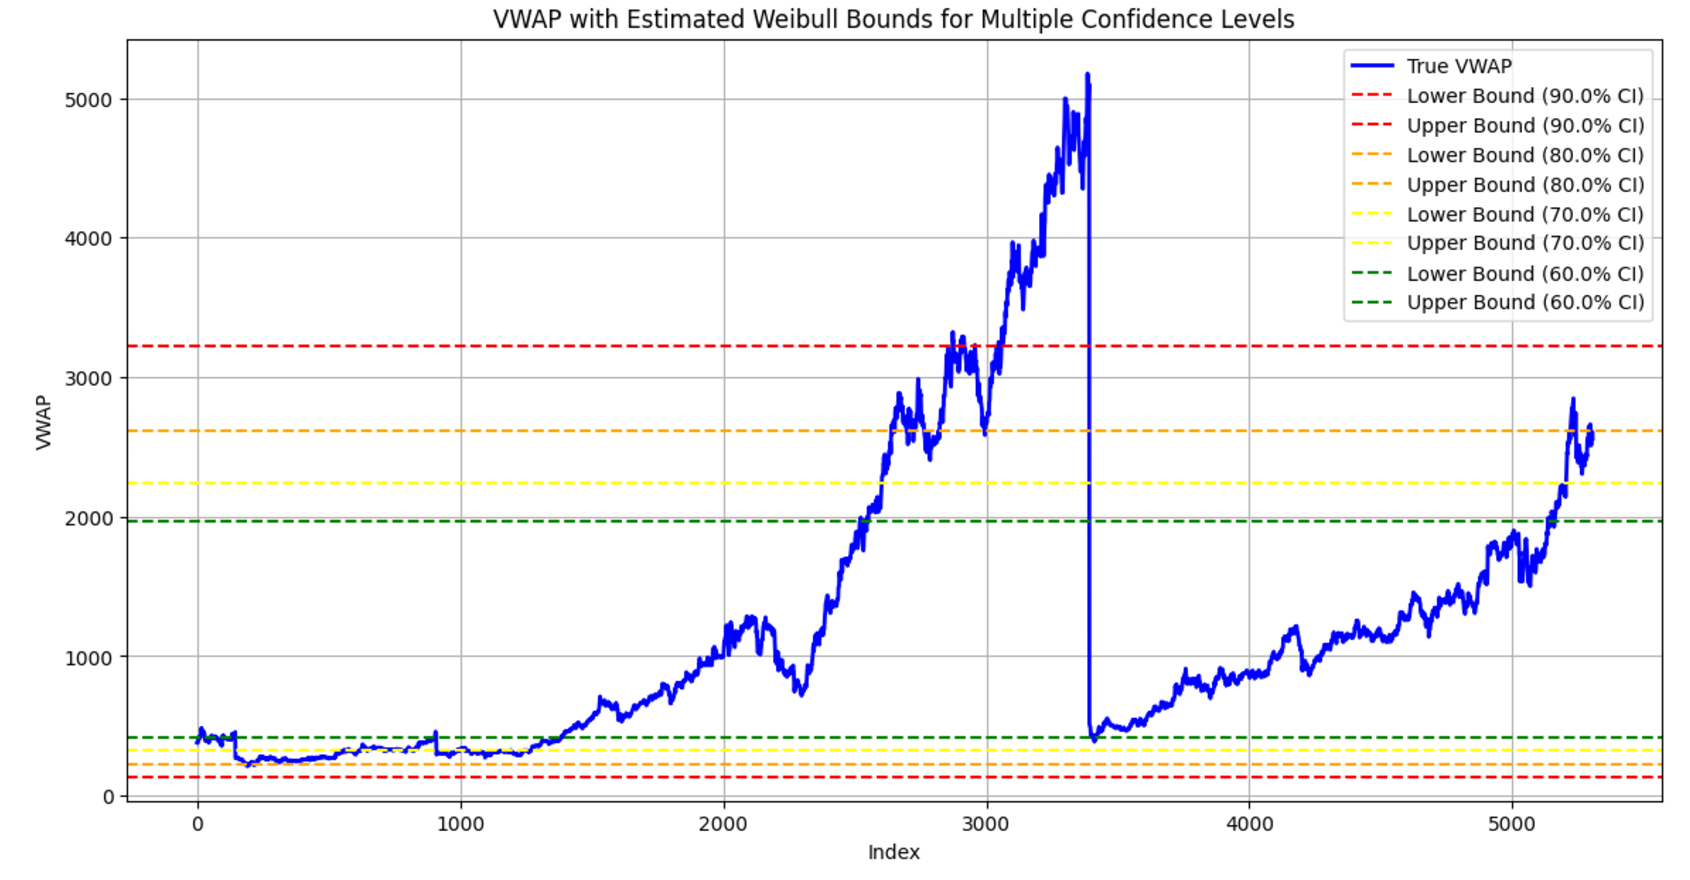
\includegraphics[width=\textwidth]{Chap02/figs/Weibull_AsianPaints.png}
                \caption{Asian Paints Dataset.}
            \end{subfigure}
            \begin{subfigure}[b]{0.8\textwidth}
                \centering
                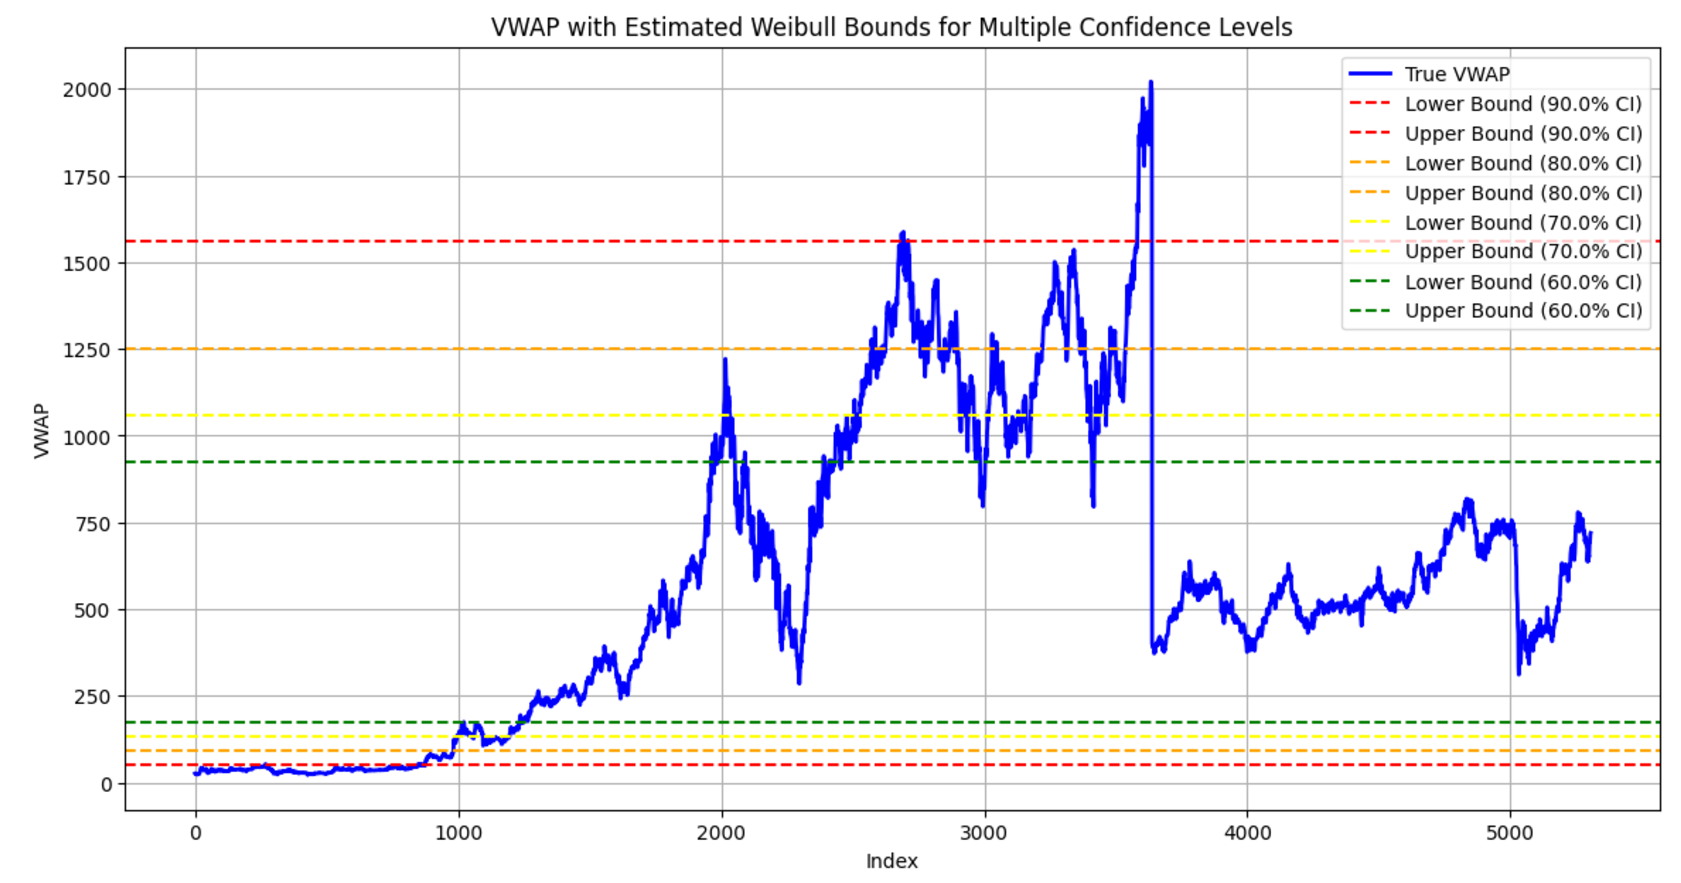
\includegraphics[width=\textwidth]{Chap02/figs/Weibull_AxisBank.png}
                \caption{Axis Bank Dataset.}
            \end{subfigure}
            \begin{subfigure}[b]{0.8\textwidth}
                \centering
                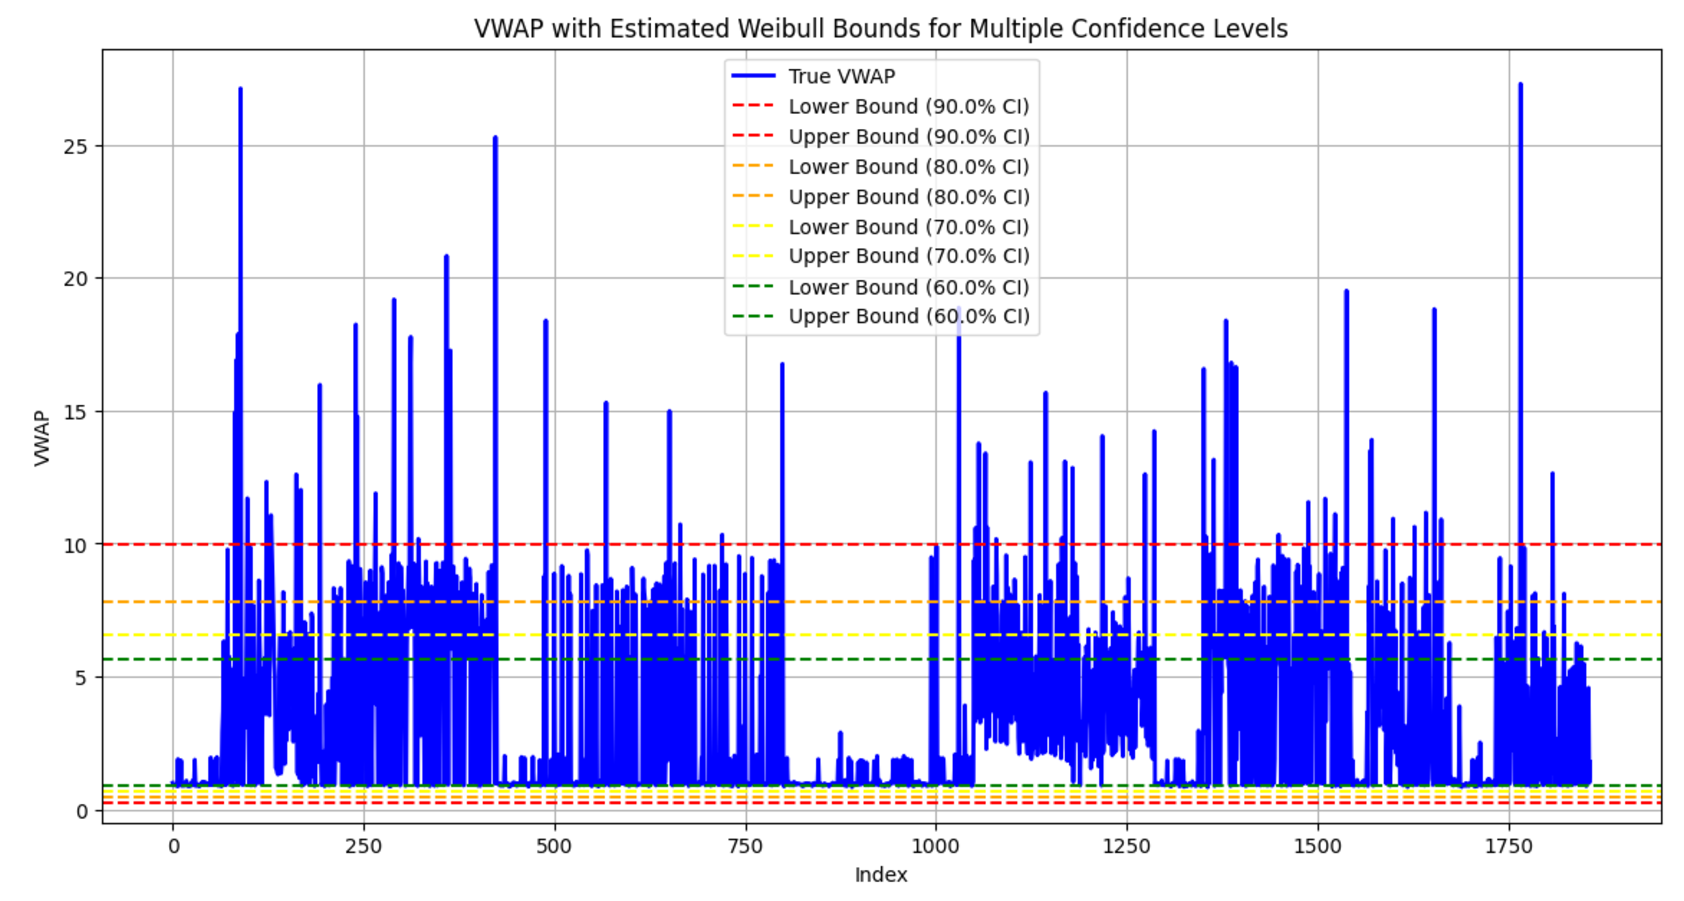
\includegraphics[width=\textwidth]{Chap02/figs/Weibull_Electricity_Consumption.png}
                \caption{Electricity Consumption Dataset.}
            \end{subfigure}

            \begin{subfigure}[b]{0.8\textwidth}
                \centering
                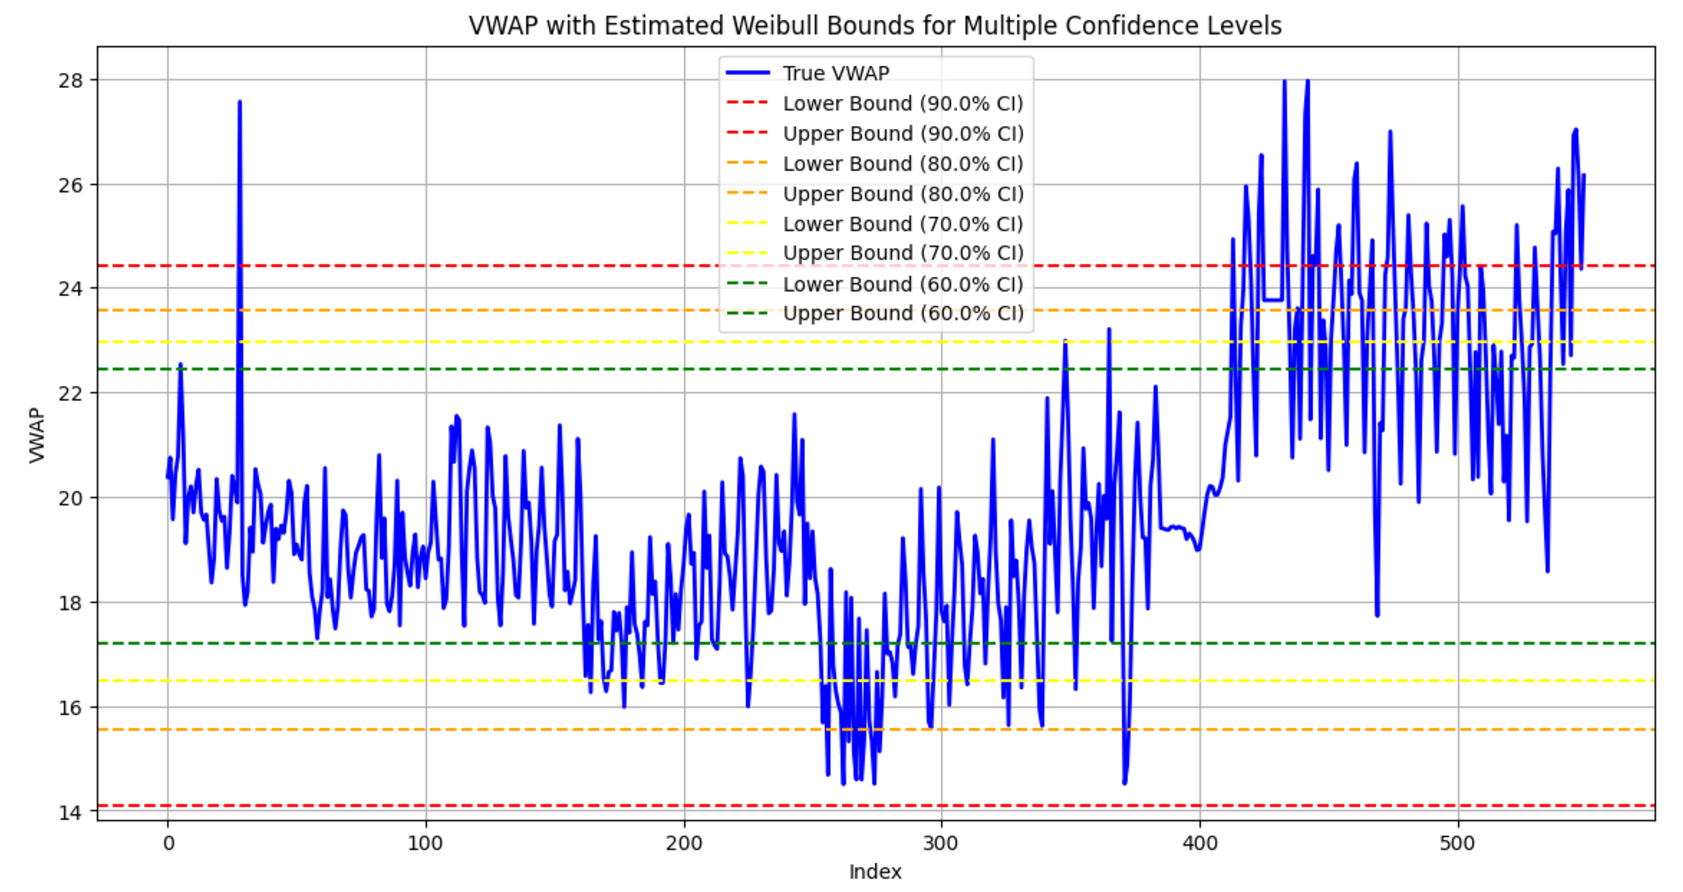
\includegraphics[width=\textwidth]{Chap02/figs/Weibull_Web_Traffic.png}
                \caption{Web Traffic Dataset.}
            \end{subfigure}
        \end{minipage}
    
    \caption{Prediction Intervals for (a) Adani Ports, (b) Asian Paints, (c) Axis Bank, (d) Electricity Consumption Load, (e) Web Traffic datasets obtained using Weibull Distribution method.}
    \label{Fi 3.7}
\end{figure}

\subsection{Discussion}
The results of this study are quite enlightening with respect to the dynamics that characterize probabilistic forecasting as well as the interactions among various methodologies and datasets. Notable in this respect is that non-parametric techniques had a tendency to vary widely in performance between datasets, indicating their effectiveness in modeling uncertainty without requiring strict assumptions about distributions. For instance, the Advanced LUBE method consistently reached an optimal balance between interval coverage and precision, hence it proved to be reliable. Nevertheless, these methods are computationally intensive and may limit their scalability in a real-time application.
In contrast, the parametric approaches presented an interesting duality: they were good at handling structured data, such as electricity consumption, but struggled to capture the complexity of noisy data, such as stock prices and web traffic. This weakness means that these methods are more suitable for domains where the underlying distributions are well defined. The Gaussian distribution was computationally efficient but struggled with coverage accuracy, whereas the Weibull distribution was more versatile across the different datasets.

Interestingly, the model architectures also had a significant role in the forecasting results. CNN and LSTM models performed very well because they are adept at capturing non-linear and temporal dependencies, while GRU and BiLSTM have mixed results, probably because of the complexity of the dataset. These findings bring out the importance of the alignment of model architecture and method selection with the data characteristics.

This research highlights the necessity for hybrid methodologies that combine the accuracy of non-parametric techniques with the effectiveness of parametric frameworks. These strategies have the potential to alleviate the computational limitations associated with non-parametric approaches while preserving adaptability. Furthermore, subsequent investigations might examine adaptive techniques that can fluidly transition between forecasting methods in response to real-time data patterns, thereby facilitating more flexible applications.

Tables \ref{Table 1} to \ref{Table 5} displays the performance of the four non-parametric methods Traditional LUBE, Advanced LUBE, QR-based and Bootstrap-based methods on the five different datasets namely Adani Ports, Asian Paints, Axis Bank, Electricity Consumption and Web Traffic. It displays the results across four evaluation metrics and four different confidence levels (90\%, 80\%, 70\% and 60\%) for each method.

Tables \ref{Table 6} to \ref{Table 10} displays the performance of two parametric methods Gaussian and Weibull Distribution based methods across four different confidence levels and four different evaluation metrics on five different datasets namely Adani Ports, Asian Paints, Axis Bank, Electricity Consumption and Web Traffic.

\newpage
\begin{table*}[!t]
\centering
\caption{Comparative Performance of LUBE, Advanced LUBE, QR-based, Bootstrap Based Methods on Adani Ports dataset.}
\vspace{0.5cm}
\renewcommand{\arraystretch}{0.8} % Adjust the value as needed
\resizebox{\textwidth}{!}{%
\begin{tabular}{|l|l|l|l|l|l|l|}
\hline
\textbf{Method Used} & \textbf{Confidence Level} & \textbf{Model} & \textbf{Avg PICP} & \textbf{Avg PINAW} &  \textbf{Avg ACE} & \textbf{Avg AWE} \\ \hline
\multirow{Traditional LUBE} & 0.6 & BiLSTM & 100 & 31.03 & 40 & 18724.39  \\ \cline{2-7}
& 0.6 & CNN & 100 & 10.07 & 40 & 5661.41 \\ \cline{2-7}
& 0.6 & GRU & 100 & 7.65 & 40 & 4148.68 \\ \cline{2-7}
& 0.6 & LSTM & 100 & 4.94 & 40 & 2460.54 \\ \cline{2-7}
& 0.7 & BiLSTM & 100 & 405.30 & 30 & 252109.41 \\ \cline{2-7}
& 0.7 & CNN & 100 & 9.93 & 30 & 5571.24 \\  \cline{2-7}
& 0.7 & GRU & 100 & 6.63 & 30 & 3513.81 \\ \cline{2-7}
& 0.7 & LSTM & 100 & 4.80 & 30 & 2369.84 \\ \cline{2-7}
& 0.8 & BiLSTM & 100 & 25.62 & 20 & 15358.03 \\ \cline{2-7}
& 0.8 & CNN & 100 & 9.96 & 20 & 5592.60 \\ \cline{2-7}
& 0.8 & GRU & 100 & 7.62 & 20 & 4128.26 \\ \cline{2-7}
& 0.8 & LSTM & 100 & 6.85 & 20 & 3652.41 \\ \cline{2-7}
& 0.9 & BiLSTM & 100 & 624.92 & 10 & 389055.75 \\ \cline{2-7}
& 0.9 & CNN & 100 & 10.01 & 10 & 5619.03 \\ \cline{2-7}
& 0.9 & GRU & 100 & 7.32 & 10 & 3942.56 \\ \cline{2-7}
& 0.9 & LSTM & 100 & 5.10 & 10 & 2557.74 \\ \hline


\multirow{Advanced LUBE} & 0.6 & BiLSTM & 100 & 6.54 & 40 & 3453.78 \\ \cline{2-7}
& 0.6 & CNN & 100 & 3.08 & 40 & 1297.77 \\ \cline{2-7}
& 0.6 & GRU & 100 & 3.21 & 40 & 1376.41 \\ \cline{2-7}
& 0.6 & LSTM & 100 & 6.21 & 40 & 3247.55 \\ \cline{2-7}
& 0.7 & BiLSTM & 100 & 7.18 & 30 & 3854.64 \\ \cline{2-7}
& 0.7 & CNN & 100 & 3.05 & 30 & 1278.93 \\ \cline{2-7}
& 0.7 & GRU & 100 & 3.34 & 30 & 1459.42 \\ \cline{2-7}
& 0.7 & LSTM & 100 & 6.02 & 30 & 3129.68 \\ \cline{2-7}
& 0.8 & BiLSTM & 100 & 6.85 & 20 & 3649.99 \\ \cline{2-7}
& 0.8 & CNN & 100 & 3.14 & 20 & 1333.73 \\ \cline{2-7}
& 0.8 & GRU & 100 & 3.06 & 20 & 1287.54 \\ \cline{2-7}
& 0.8 & LSTM & 100 & 6.90 & 20 & 3676.17 \\ \cline{2-7}
& 0.9 & BiLSTM & 100 & 6.61 & 10 & 3497.79 \\ \cline{2-7}
& 0.9 & CNN & 100 & 3.08 & 10 & 1297.10 \\ \cline{2-7}
& 0.9 & GRU & 100 & 3.47 & 10 & 1537.40 \\ \cline{2-7}
& 0.9 & LSTM & 100 & 6.94 & 10 & 3702.24 \\ \hline


\multirow{QR-based} & 0.6 & BiLSTM & 67.87 & 0.03 & 12.36 & 607.25 \\ \cline{2-7}
& 0.6 & CNN & 79.07 & 0.10 & 21.86 & 562.45 \\ \cline{2-7}
& 0.6 & GRU & 58.87 & 0.02 & 21.24 & 608.68 \\ \cline{2-7}
& 0.6 & LSTM & 70.68 & 0.04 & 26.97 & 600.36 \\ \cline{2-7}
& 0.7 & BiLSTM & 60.72 & 0.03 & 21.29 & 606.88 \\ \cline{2-7}
& 0.7 & CNN & 86.96 & 0.11 & 16.96 & 551.85 \\ \cline{2-7}
& 0.7 & GRU & 72.49 & 0.04 & 21.80 & 601.08 \\ \cline{2-7}
& 0.7 & LSTM & 67.38 & 0.03 & 21.79 & 602.06 \\ \cline{2-7}
& 0.8 & BiLSTM & 86.72 & 0.06 & 8.42 & 587.38 \\ \cline{2-7}
& 0.8 & CNN & 86.74 & 0.13 & 12.12 & 539.85 \\ \cline{2-7}
& 0.8 & GRU & 82.27 & 0.04 & 9.11 & 598.12 \\ \cline{2-7}
& 0.8 & LSTM & 80.08 & 0.06 & 13.03 & 589.16 \\ \cline{2-7}
& 0.9 & BiLSTM & 94.55 & 0.08 & 5.69 & 572.07 \\ \cline{2-7}
& 0.9 & CNN & 95.73 & 0.19 & 5.75 & 507.37 \\ \cline{2-7}
& 0.9 & GRU & 89.80 & 0.07 & 9.49 & 577.76 \\ \cline{2-7}
& 0.9 & LSTM & 97.08 & 0.10 & 7.30 & 561.57 \\ \hline

\multirow{Bootstrap-based} & 0.6 & BiLSTM & 57.48 & 0.17 & 2.55 & 519.87 \\ \cline{2-7}
& 0.6 & CNN & 56.58 & 0.16 & 3.92 & 521.28 \\ \cline{2-7}
& 0.6 & GRU & 58.95 & 0.17 & 2.17 & 519.90 \\ \cline{2-7}
& 0.6 & LSTM & 57.81 & 0.17 & 2.31 & 519.69 \\ \cline{2-7}
& 0.7 & BiLSTM & 67.97 & 0.27 & 2.08 & 453.09 \\ \cline{2-7}
& 0.7 & CNN & 67.34 & 0.28 & 3.03 & 450.21 \\ \cline{2-7}
& 0.7 & GRU & 68.43 & 0.28 & 1.65 & 451.96 \\ \cline{2-7}
& 0.7 & LSTM & 65.88 & 0.27 & 4.17 & 454.46 \\ \cline{2-7}
& 0.8 & BiLSTM & 76.62 & 0.45 & 3.38 & 340.08 \\ \cline{2-7}
& 0.8 & CNN & 77.04 & 0.45 & 3.13 & 341.60 \\ \cline{2-7}
& 0.8 & GRU & 78.29 & 0.46 & 1.71 & 337.02 \\ \cline{2-7}
& 0.8 & LSTM & 78.27 & 0.46 & 1.87 & 338.39 \\ \cline{2-7}
& 0.9 & BiLSTM & 87.53 & 0.68 & 2.47 & 199.80 \\ \cline{2-7}
& 0.9 & CNN & 88.19 & 0.69 & 2.08 & 190.55 \\ \cline{2-7}
& 0.9 & GRU & 88.05 & 0.68 & 1.95 & 198.01 \\ \cline{2-7}
& 0.9 & LSTM & 87.67 & 0.68 & 2.33 & 199.72 \\ \hline
\end{tabular}%
}
\label{Table 1}
\end{table*}

\begin{table*}[!t]
\centering
\caption{Comparative Performance of LUBE, Advanced LUBE, QR-based, Bootstrap Based Methods on Asian Paints dataset.}
\vspace{0.5cm}
\renewcommand{\arraystretch}{0.8} % Adjust the value as needed
\resizebox{\textwidth}{!}{%
\begin{tabular}{|l|l|l|l|l|l|l|}
\hline
\textbf{Method Used} & \textbf{Confidence Level} & \textbf{Model} & \textbf{Avg PICP} & \textbf{Avg PINAW} &  \textbf{Avg ACE} & \textbf{Avg AWE} \\ \hline
\multirow{Traditional LUBE} 
& 0.6 & BiLSTM & 100 & 176.2462 & 40 & 306120.048 \\ \cline{2-7}
& 0.6 & CNN & 100 & 16.7941 & 40 & 27589.0975 \\ \cline{2-7}
& 0.6 & GRU & 100 & 8.7152 & 40 & 13476.9307 \\ \cline{2-7}
& 0.6 & LSTM & 100 & 6.3460 & 40 & 9338.4101 \\ \cline{2-7}
& 0.7 & BiLSTM & 100 & 134.8771 & 30 & 233856.5168 \\ \cline{2-7}
& 0.7 & CNN & 100 & 16.4525 & 30 & 26992.4830 \\ \cline{2-7}
& 0.7 & GRU & 100 & 8.4597 & 30 & 13030.5229 \\ \cline{2-7}
& 0.7 & LSTM & 100 & 6.3955 & 30 & 9424.8555 \\ \cline{2-7}
& 0.8 & BiLSTM & 100 & 107.5393 & 20 & 186102.8086 \\ \cline{2-7}
& 0.8 & CNN & 100 & 16.6753 & 20 & 27381.5852 \\ \cline{2-7}
& 0.8 & GRU & 100 & 8.4415 & 20 & 12998.7874 \\ \cline{2-7}
& 0.8 & LSTM & 100 & 6.4796 & 20 & 9571.7360 \\ \cline{2-7}
& 0.9 & BiLSTM & 100 & 82.2330 & 10 & 141897.7734 \\ \cline{2-7}
& 0.9 & CNN & 100 & 17.2459 & 10 & 28378.3252 \\ \cline{2-7}
& 0.9 & GRU & 100 & 8.8828 & 10 & 13769.6257 \\ \cline{2-7}
& 0.9 & LSTM & 100 & 5.8771 & 10 & 8519.3438 \\ \hline

\multirow{Advanced LUBE} & 0.6 & BiLSTM & 100 & 21.38 & 40 & 35595.10 \\ \cline{2-7}
& 0.6 & CNN & 100 & 4.87 & 40 & 6758.33 \\ \cline{2-7}
& 0.6 & GRU & 100 & 6.44 & 40 & 9493.89 \\ \cline{2-7}
& 0.6 & LSTM & 100 & 11.99 & 40 & 19192.37 \\ \cline{2-7}
& 0.7 & BiLSTM & 100 & 19.89 & 30 & 32988.48 \\ \cline{2-7}
& 0.7 & CNN & 100 & 5.12 & 30 & 7205.28 \\ \cline{2-7}
& 0.7 & GRU & 100 & 6.58 & 30 & 9740.53 \\ \cline{2-7}
& 0.7 & LSTM & 100 & 12.73 & 30 & 20486.20 \\ \cline{2-7}
& 0.8 & BiLSTM & 100 & 18.56 & 20 & 30669.12 \\ \cline{2-7}
& 0.8 & CNN & 100 & 5.04 & 20 & 7062.18 \\ \cline{2-7}
& 0.8 & GRU & 100 & 6.77 & 20 & 10078.24 \\ \cline{2-7}
& 0.8 & LSTM & 100 & 12.21 & 20 & 19584.56 \\ \cline{2-7}
& 0.9 & BiLSTM & 100 & 16.27 & 10 & 26678.04 \\ \cline{2-7}
& 0.9 & CNN & 100 & 5.24 & 10 & 7401.71 \\ \cline{2-7}
& 0.9 & GRU & 100 & 6.20 & 10 & 9086.57 \\ \cline{2-7}
& 0.9 & LSTM & 100 & 13.03 & 10 & 21021.77 \\ \hline

\multirow{QR-based} & 0.6 & BiLSTM & 49.45 & 0.03 & 22.91 & 1702.05 \\ \cline{2-7}
& 0.6 & CNN & 81.00 & 0.13 & 23.66 & 1518.25 \\ \cline{2-7}
& 0.6 & GRU & 35.04 & 0.01 & 33.01 & 1720.67 \\ \cline{2-7}
& 0.6 & LSTM & 39.30 & 0.02 & 35.72 & 1709.96 \\ \cline{2-7}
& 0.7 & BiLSTM & 57.99 & 0.03 & 17.33 & 1689.08 \\ \cline{2-7}
& 0.7 & CNN & 95.28 & 0.20 & 25.28 & 1402.63 \\ \cline{2-7}
& 0.7 & GRU & 52.10 & 0.02 & 26.34 & 1706.18 \\ \cline{2-7}
& 0.7 & LSTM & 74.25 & 0.04 & 18.81 & 1670.70 \\ \cline{2-7}
& 0.8 & BiLSTM & 68.73 & 0.04 & 20.23 & 1670.69 \\ \cline{2-7}
& 0.8 & CNN & 94.19 & 0.21 & 16.91 & 1380.19 \\ \cline{2-7}
& 0.8 & GRU & 81.57 & 0.05 & 9.77 & 1661.94 \\ \cline{2-7}
& 0.8 & LSTM & 79.16 & 0.06 & 19.18 & 1638.10 \\ \cline{2-7}
& 0.9 & BiLSTM & 88.19 & 0.06 & 10.38 & 1637.48 \\ \cline{2-7}
& 0.9 & CNN & 98.68 & 0.32 & 8.68 & 1185.35 \\ \cline{2-7}
& 0.9 & GRU & 84.93 & 0.07 & 9.97 & 1632.32 \\ \cline{2-7}
& 0.9 & LSTM & 71.18 & 0.06 & 23.80 & 1645.33 \\ \hline

\multirow{Bootstrap-based} & 0.6 & BiLSTM & 59.51 & 0.37 & 1.12 & 1102.74 \\ \cline{2-7}
& 0.6 & CNN & 56.96 & 0.37 & 4.45 & 1098.73 \\ \cline{2-7}
& 0.6 & GRU & 58.70 & 0.36 & 1.80 & 1111.23 \\ \cline{2-7}
& 0.6 & LSTM & 57.26 & 0.36 & 3.85 & 1110.84 \\ \cline{2-7}
& 0.7 & BiLSTM & 68.73 & 0.49 & 1.50 & 884.40 \\ \cline{2-7}
& 0.7 & CNN & 67.72 & 0.49 & 3.99 & 892.03 \\ \cline{2-7}
& 0.7 & GRU & 69.01 & 0.49 & 1.35 & 885.19 \\ \cline{2-7}
& 0.7 & LSTM & 69.07 & 0.49 & 1.46 & 885.54 \\ \cline{2-7}
& 0.8 & BiLSTM & 77.19 & 0.63 & 2.81 & 646.05 \\ \cline{2-7}
& 0.8 & CNN & 79.03 & 0.65 & 1.50 & 611.55 \\ \cline{2-7}
& 0.8 & GRU & 78.91 & 0.64 & 1.35 & 627.15 \\ \cline{2-7}
& 0.8 & LSTM & 79.01 & 0.64 & 1.07 & 621.64 \\ \cline{2-7}
& 0.9 & BiLSTM & 89.08 & 0.79 & 1.28 & 369.51 \\ \cline{2-7}
& 0.9 & CNN & 88.31 & 0.78 & 2.19 & 383.92 \\ \cline{2-7}
& 0.9 & GRU & 88.70 & 0.79 & 1.30 & 373.43 \\ \cline{2-7}
& 0.9 & LSTM & 89.48 & 0.79 & 0.97 & 369.39 \\ \hline
\end{tabular}%
}
\label{Table 2}
\end{table*}

\begin{table*}[!t]
\centering
\caption{Comparative Performance of LUBE, Advanced LUBE, QR-based, Bootstrap Based Methods on Axis Bank dataset.}
\vspace{0.5cm}
\renewcommand{\arraystretch}{0.8} % Adjust the value as needed
\resizebox{\textwidth}{!}{%
\begin{tabular}{|l|l|l|l|l|l|l|}
\hline
\textbf{Method Used} & \textbf{Confidence Level} & \textbf{Model} & \textbf{Avg PICP} & \textbf{Avg PINAW} &  \textbf{Avg ACE} & \textbf{Avg AWE} \\ \hline
\multirow{Traditional LUBE} & 0.6 & BiLSTM & 100 & 142.23 & 40 & 71594.44 \\ \cline{2-7}
& 0.6 & CNN & 100 & 21.70 & 40 & 10492.69 \\ \cline{2-7}
& 0.6 & GRU & 100 & 13.41 & 40 & 6290.57 \\ \cline{2-7}
& 0.6 & LSTM & 100 & 10.36 & 40 & 4746.86 \\ \cline{2-7}
& 0.7 & BiLSTM & 100 & 84.23 & 30 & 42192.68 \\ \cline{2-7}
& 0.7 & CNN & 100 & 21.98 & 30 & 10635.94 \\ \cline{2-7}
& 0.7 & GRU & 100 & 14.67 & 30 & 6932.03 \\ \cline{2-7}
& 0.7 & LSTM & 100 & 8.15 & 30 & 3623.44 \\ \cline{2-7}
& 0.8 & BiLSTM & 100 & 30683.37 & 20 & 15554427.52 \\ \cline{2-7}
& 0.8 & CNN & 100 & 22.58 & 20 & 10939.10 \\ \cline{2-7}
& 0.8 & GRU & 100 & 15.97 & 20 & 7587.76 \\ \cline{2-7}
& 0.8 & LSTM & 100 & 9.98 & 20 & 4553.34 \\ \cline{2-7}
& 0.9 & BiLSTM & 100 & 110.06 & 10 & 55289.93 \\ \cline{2-7}
& 0.9 & CNN & 100 & 22.11 & 10 & 10700.12 \\ \cline{2-7}
& 0.9 & GRU & 100 & 16.70 & 10 & 7957.61 \\ \cline{2-7}
& 0.9 & LSTM & 100 & 10.35 & 10 & 4741.71 \\ \hline

\multirow{Advanced LUBE} & 0.6 & BiLSTM & 100 & 19.02 & 40 & 9136.65 \\ \cline{2-7}
& 0.6 & CNN & 100 & 6.97 & 40 & 3027.38 \\ \cline{2-7}
& 0.6 & GRU & 100 & 7.53 & 40 & 3311.35 \\ \cline{2-7}
& 0.6 & LSTM & 100 & 15.30 & 40 & 7248.18 \\ \cline{2-7}
& 0.7 & BiLSTM & 100 & 17.66 & 30 & 8445.44 \\ \cline{2-7}
& 0.7 & CNN & 100 & 7.11 & 30 & 3098.77 \\ \cline{2-7}
& 0.7 & GRU & 100 & 7.49 & 30 & 3287.88 \\ \cline{2-7}
& 0.7 & LSTM & 100 & 14.99 & 30 & 7091.83 \\ \cline{2-7}
& 0.8 & BiLSTM & 100 & 19.64 & 20 & 9449.07 \\ \cline{2-7}
& 0.8 & CNN & 100 & 6.86 & 20 & 2972.82 \\ \cline{2-7}
& 0.8 & GRU & 100 & 7.77 & 20 & 3432.81 \\ \cline{2-7}
& 0.8 & LSTM & 100 & 15.69 & 20 & 7448.36 \\ \cline{2-7}
& 0.9 & BiLSTM & 100 & 21.82 & 10 & 10554.26 \\ \cline{2-7}
& 0.9 & CNN & 100 & 6.64 & 10 & 2861.38 \\ \cline{2-7}
& 0.9 & GRU & 100 & 7.10 & 10 & 3094.89 \\ \cline{2-7}
& 0.9 & LSTM & 100 & 16.27 & 10 & 7743.09 \\ \hline

\multirow{QR-based} & 0.6 & BiLSTM & 63.97 & 0.05 & 16.28 & 481.88 \\ \cline{2-7}
& 0.6 & CNN & 78.04 & 0.17 & 25.41 & 423.17 \\ \cline{2-7}
& 0.6 & GRU & 74.13 & 0.06 & 16.84 & 476.30 \\ \cline{2-7}
& 0.6 & LSTM & 81.17 & 0.09 & 24.06 & 460.57 \\ \cline{2-7}
& 0.7 & BiLSTM & 82.44 & 0.08 & 18.72 & 466.64 \\ \cline{2-7}
& 0.7 & CNN & 93.64 & 0.24 & 23.64 & 384.16 \\ \cline{2-7}
& 0.7 & GRU & 78.98 & 0.07 & 11.27 & 472.55 \\ \cline{2-7}
& 0.7 & LSTM & 87.99 & 0.11 & 20.52 & 453.45 \\ \cline{2-7}
& 0.8 & BiLSTM & 86.69 & 0.09 & 8.15 & 459.56 \\ \cline{2-7}
& 0.8 & CNN & 96.35 & 0.30 & 16.35 & 355.55 \\ \cline{2-7}
& 0.8 & GRU & 88.24 & 0.09 & 8.89 & 462.92 \\ \cline{2-7}
& 0.8 & LSTM & 84.69 & 0.09 & 14.30 & 461.12 \\ \cline{2-7}
& 0.9 & BiLSTM & 96.65 & 0.15 & 6.74 & 429.74 \\ \cline{2-7}
& 0.9 & CNN & 98.25 & 0.41 & 8.25 & 299.18 \\ \cline{2-7}
& 0.9 & GRU & 95.96 & 0.17 & 7.53 & 423.20 \\ \cline{2-7}
& 0.9 & LSTM & 89.23 & 0.13 & 9.45 & 442.80 \\ \hline

\multirow{Bootstrap-based} & 0.6 & BiLSTM & 59.80 & 0.47 & 2.19 & 268.87 \\ \cline{2-7}
& 0.6 & CNN & 61.04 & 0.47 & 2.96 & 267.34 \\ \cline{2-7}
& 0.6 & GRU & 60.68 & 0.47 & 1.79 & 269.28 \\ \cline{2-7}
& 0.6 & LSTM & 59.50 & 0.47 & 2.31 & 269.05 \\ \cline{2-7}
& 0.7 & BiLSTM & 70.53 & 0.56 & 1.91 & 224.65 \\ \cline{2-7}
& 0.7 & CNN & 71.46 & 0.56 & 2.96 & 220.82 \\ \cline{2-7}
& 0.7 & GRU & 72.65 & 0.56 & 2.97 & 224.17 \\ \cline{2-7}
& 0.7 & LSTM & 68.44 & 0.55 & 2.84 & 226.77 \\ \cline{2-7}
& 0.8 & BiLSTM & 79.60 & 0.63 & 1.36 & 188.36 \\ \cline{2-7}
& 0.8 & CNN & 73.03 & 0.62 & 7.17 & 191.75 \\ \cline{2-7}
& 0.8 & GRU & 80.23 & 0.63 & 0.91 & 186.70 \\ \cline{2-7}
& 0.8 & LSTM & 79.46 & 0.63 & 1.17 & 186.19 \\ \cline{2-7}
& 0.9 & BiLSTM & 88.88 & 0.72 & 1.12 & 142.82 \\ \cline{2-7}
& 0.9 & CNN & 87.50 & 0.72 & 2.50 & 140.65 \\ \cline{2-7}
& 0.9 & GRU & 88.87 & 0.72 & 1.13 & 142.78 \\ \cline{2-7}
& 0.9 & LSTM & 85.02 & 0.71 & 4.98 & 148.03 \\ \hline

\end{tabular}%
}
\label{Table 3}
\end{table*}

\begin{table*}[!t]
\centering
\caption{Comparative Performance of LUBE, Advanced LUBE, QR-based, Bootstrap Based Methods on Electricity Consumption dataset.}
\vspace{0.5cm}
\renewcommand{\arraystretch}{0.8} % Adjust the value as needed
\resizebox{\textwidth}{!}{%
\begin{tabular}{|l|l|l|l|l|l|l|}
\hline
\textbf{Method Used} & \textbf{Confidence Level} & \textbf{Model} & \textbf{Avg PICP} & \textbf{Avg PINAW} &  \textbf{Avg ACE} & \textbf{Avg AWE} \\ \hline

\multirow{Traditional LUBE} & 0.6 & BiLSTM & 100.00 & 3.69 & 40 & 71.06 \\ \cline{2-7}
& 0.6 & CNN & 100.00 & 4.15 & 40 & 83.35 \\ \cline{2-7}
& 0.6 & GRU & 100.00 & 2.44 & 40 & 38.01 \\ \cline{2-7}
& 0.6 & LSTM & 100.00 & 2.24 & 40 & 32.70 \\ \cline{2-7}
& 0.7 & BiLSTM & 100.00 & 3.80 & 30 & 74.14 \\ \cline{2-7}
& 0.7 & CNN & 100.00 & 4.00 & 30 & 79.19 \\ \cline{2-7}
& 0.7 & GRU & 100.00 & 1.70 & 30 & 18.59 \\ \cline{2-7}
& 0.7 & LSTM & 100.00 & 2.68 & 30 & 44.36 \\ \cline{2-7}
& 0.8 & BiLSTM & 100.00 & 5.71 & 20 & 124.41 \\ \cline{2-7}
& 0.8 & CNN & 100.00 & 4.10 & 20 & 82.06 \\ \cline{2-7}
& 0.8 & GRU & 100.00 & 2.81 & 20 & 47.74 \\ \cline{2-7}
& 0.8 & LSTM & 100.00 & 2.75 & 20 & 46.31 \\ \cline{2-7}
& 0.9 & BiLSTM & 100.00 & 4.16 & 10 & 83.67 \\ \cline{2-7}
& 0.9 & CNN & 100.00 & 4.19 & 10 & 84.42 \\ \cline{2-7}
& 0.9 & GRU & 100.00 & 2.25 & 10 & 33.16 \\ \cline{2-7}
& 0.9 & LSTM & 100.00 & 1.97 & 10 & 25.68 \\ \hline



\multirow{Advanced LUBE} 
& 0.6 & BiLSTM & 100.00 & 2.02 & 40 & 27.09 \\ \cline{2-7}
& 0.6 & CNN & 99.68 & 0.99 & 39.68 & 0.90 \\ \cline{2-7}
& 0.6 & GRU & 100.00 & 1.39 & 40 & 10.31 \\ \cline{2-7}
& 0.6 & LSTM & 100.00 & 2.07 & 40 & 28.23 \\ \cline{2-7}
& 0.7 & BiLSTM & 100.00 & 1.82 & 30 & 21.70 \\ \cline{2-7}
& 0.7 & CNN & 99.67 & 0.99 & 29.67 & 0.65 \\ \cline{2-7}
& 0.7 & GRU & 100.00 & 1.48 & 30 & 12.79 \\ \cline{2-7}
& 0.7 & LSTM & 100.00 & 1.98 & 30 & 25.95 \\ \cline{2-7}
& 0.8 & BiLSTM & 100.00 & 1.99 & 20 & 26.15 \\ \cline{2-7}
& 0.8 & CNN & 99.67 & 0.98 & 19.67 & 1.08 \\ \cline{2-7}
& 0.8 & GRU & 100.00 & 1.36 & 20 & 9.52 \\ \cline{2-7}
& 0.8 & LSTM & 100.00 & 2.32 & 20 & 35.01 \\ \cline{2-7}
& 0.9 & BiLSTM & 100.00 & 1.66 & 10 & 17.32 \\ \cline{2-7}
& 0.9 & CNN & 99.69 & 1.01 & 9.69 & 0.92 \\ \cline{2-7}
& 0.9 & GRU & 100.00 & 1.35 & 10 & 9.32 \\ \cline{2-7}
& 0.9 & LSTM & 100.00 & 2.21 & 10 & 32.04 \\ \hline


\multirow{QR-based} 
& 0.6 & BiLSTM & 46.69 & 0.1443 & 13.31 & 22.63 \\ \cline{2-7}
& 0.6 & CNN & 56.94 & 0.1667 & 10.44 & 22.03 \\ \cline{2-7}
& 0.6 & GRU & 50.04 & 0.1494 & 10.70 & 22.49 \\ \cline{2-7}
& 0.6 & LSTM & 65.47 & 0.1605 & 12.68 & 22.20 \\ \cline{2-7}
& 0.7 & BiLSTM & 70.76 & 0.1980 & 4.37 & 21.21 \\ \cline{2-7}
& 0.7 & CNN & 73.78 & 0.2004 & 4.11 & 21.14 \\ \cline{2-7}
& 0.7 & GRU & 65.61 & 0.1838 & 10.45 & 21.58 \\ \cline{2-7}
& 0.7 & LSTM & 74.86 & 0.1997 & 12.18 & 21.16 \\ \cline{2-7}
& 0.8 & BiLSTM & 78.92 & 0.2372 & 6.69 & 20.17 \\ \cline{2-7}
& 0.8 & CNN & 82.73 & 0.2484 & 5.94 & 19.87 \\ \cline{2-7}
& 0.8 & GRU & 81.98 & 0.2278 & 5.22 & 20.42 \\ \cline{2-7}
& 0.8 & LSTM & 81.51 & 0.2473 & 10.86 & 19.90 \\ \cline{2-7}
& 0.9 & BiLSTM & 88.35 & 0.2900 & 4.82 & 18.77 \\ \cline{2-7}
& 0.9 & CNN & 87.52 & 0.3027 & 5.66 & 18.44 \\ \cline{2-7}
& 0.9 & GRU & 90.65 & 0.3133 & 3.58 & 18.16 \\ \cline{2-7}
& 0.9 & LSTM & 83.96 & 0.3342 & 15.01 & 17.60 \\ \hline


\multirow{Bootstrap-based} 
& 0.6 & BiLSTM & 24.42 & 0.0846 & 35.58 & 24.20 \\ \cline{2-7}
& 0.6 & CNN & 24.42 & 0.0734 & 35.58 & 24.50 \\ \cline{2-7}
& 0.6 & GRU & 19.50 & 0.0777 & 40.50 & 24.39 \\ \cline{2-7}
& 0.6 & LSTM & 21.01 & 0.0762 & 38.99 & 24.43 \\ \cline{2-7}
& 0.7 & BiLSTM & 28.06 & 0.1064 & 41.94 & 23.63 \\ \cline{2-7}
& 0.7 & CNN & 32.23 & 0.0930 & 37.77 & 23.98 \\ \cline{2-7}
& 0.7 & GRU & 28.20 & 0.1040 & 41.80 & 23.69 \\ \cline{2-7}
& 0.7 & LSTM & 33.92 & 0.1029 & 36.08 & 23.72 \\ \cline{2-7}
& 0.8 & BiLSTM & 34.60 & 0.1198 & 45.40 & 23.27 \\ \cline{2-7}
& 0.8 & CNN & 32.70 & 0.1157 & 47.30 & 23.38 \\ \cline{2-7}
& 0.8 & GRU & 31.76 & 0.1152 & 48.24 & 23.39 \\ \cline{2-7}
& 0.8 & LSTM & 37.70 & 0.1184 & 42.30 & 23.31 \\ \cline{2-7}
& 0.9 & BiLSTM & 45.04 & 0.1376 & 44.96 & 22.80 \\ \cline{2-7}
& 0.9 & CNN & 43.88 & 0.1316 & 46.12 & 22.96 \\ \cline{2-7}
& 0.9 & GRU & 41.40 & 0.1335 & 48.60 & 22.91 \\ \cline{2-7}
& 0.9 & LSTM & 52.59 & 0.1297 & 37.41 & 23.01 \\ \hline

\end{tabular}%
}
\label{Table 4}
\end{table*}


\begin{table*}[!t]
\centering
\caption{Comparative Performance of LUBE, Advanced LUBE, QR-based, Bootstrap Based Methods on Web Traffic dataset.}
\vspace{0.5cm}
\renewcommand{\arraystretch}{0.8} % Adjust the value as needed
\resizebox{\textwidth}{!}{%
\begin{tabular}{|l|l|l|l|l|l|l|}
\hline
\textbf{Method Used} & \textbf{Confidence Level} & \textbf{Model} & \textbf{Avg PICP} & \textbf{Avg PINAW} &  \textbf{Avg ACE} & \textbf{Avg AWE} \\ \hline

\multirow{Traditional LUBE} 
& 0.6 & BiLSTM & 100 & 10.5871 & 40 & 89.2555 \\ \cline{2-7}
& 0.6 & CNN & 100 & 5.3765 & 40 & 40.7450 \\ \cline{2-7}
& 0.6 & GRU & 100 & 3.9920 & 40 & 27.8559 \\ \cline{2-7}
& 0.6 & LSTM & 100 & 3.7757 & 40 & 25.8415 \\ \cline{2-7}
& 0.7 & BiLSTM & 100 & 10.0964 & 30 & 84.6871 \\ \cline{2-7}
& 0.7 & CNN & 100 & 5.2022 & 30 & 39.1221 \\ \cline{2-7}
& 0.7 & GRU & 100 & 4.0640 & 30 & 28.5260 \\ \cline{2-7}
& 0.7 & LSTM & 100 & 2.8798 & 30 & 17.5013 \\ \cline{2-7}
& 0.8 & BiLSTM & 100 & 10.1790 & 20 & 85.4565 \\ \cline{2-7}
& 0.8 & CNN & 100 & 5.2952 & 20 & 39.9882 \\ \cline{2-7}
& 0.8 & GRU & 100 & 4.1002 & 20 & 28.8626 \\ \cline{2-7}
& 0.8 & LSTM & 100 & 4.0289 & 20 & 28.1994 \\ \cline{2-7}
& 0.9 & BiLSTM & 100 & 10.4536 & 10 & 88.0132 \\ \cline{2-7}
& 0.9 & CNN & 100 & 5.2567 & 10 & 39.6294 \\ \cline{2-7}
& 0.9 & GRU & 100 & 4.0724 & 10 & 28.6041 \\ \cline{2-7}
& 0.9 & LSTM & 100 & 3.7530 & 10 & 25.6306 \\ \hline

\multirow{Advanced LUBE} 
& 0.6 & BiLSTM & 100 & 5.1715 & 40 & 38.8365 \\ \cline{2-7}
& 0.6 & CNN & 99.9628 & 1.8441 & 39.9628 & 7.8588 \\ \cline{2-7}
& 0.6 & GRU & 100 & 2.9044 & 40 & 17.7303 \\ \cline{2-7}
& 0.6 & LSTM & 100 & 4.5065 & 40 & 32.6452 \\ \cline{2-7}
& 0.7 & BiLSTM & 100 & 4.6309 & 30 & 33.8035 \\ \cline{2-7}
& 0.7 & CNN & 98.9218 & 1.7859 & 28.9218 & 7.3169 \\ \cline{2-7}
& 0.7 & GRU & 100 & 3.1460 & 30 & 19.9797 \\ \cline{2-7}
& 0.7 & LSTM & 100 & 4.1576 & 30 & 29.3974 \\ \cline{2-7}
& 0.8 & BiLSTM & 100 & 5.0116 & 20 & 37.3477 \\ \cline{2-7}
& 0.8 & CNN & 99.4170 & 1.7916 & 19.4170 & 7.3702 \\ \cline{2-7}
& 0.8 & GRU & 100 & 3.0457 & 20 & 19.0454 \\ \cline{2-7}
& 0.8 & LSTM & 100 & 4.0881 & 20 & 28.7499 \\ \cline{2-7}
& 0.9 & BiLSTM & 100 & 4.9196 & 10 & 36.4912 \\ \cline{2-7}
& 0.9 & CNN & 99.1939 & 1.6862 & 9.1939 & 6.3889 \\ \cline{2-7}
& 0.9 & GRU & 100 & 3.1565 & 10 & 20.0771 \\ \cline{2-7}
& 0.9 & LSTM & 100 & 4.2867 & 10 & 30.5994 \\ \hline

\multirow{QR-based} 
& 0.6 & BiLSTM & 21.4634 & 0.2639 & 38.5366 & 6.8529 \\ \cline{2-7}
& 0.6 & CNN & 15.1220 & 0.2586 & 44.8780 & 6.9025 \\ \cline{2-7}
& 0.6 & GRU & 33.7805 & 0.3303 & 26.2195 & 6.2347 \\ \cline{2-7}
& 0.6 & LSTM & 19.6341 & 0.2617 & 40.3659 & 6.8733 \\ \cline{2-7}
& 0.7 & BiLSTM & 25.8537 & 0.3031 & 44.1463 & 6.4879 \\ \cline{2-7}
& 0.7 & CNN & 18.4146 & 0.3330 & 51.5854 & 6.2101 \\ \cline{2-7}
& 0.7 & GRU & 43.2927 & 0.3703 & 26.7073 & 5.8625 \\ \cline{2-7}
& 0.7 & LSTM & 25.2439 & 0.2937 & 44.7561 & 6.5756 \\ \cline{2-7}
& 0.8 & BiLSTM & 50.2439 & 0.4557 & 29.7561 & 5.0670 \\ \cline{2-7}
& 0.8 & CNN & 24.3902 & 0.4074 & 55.6098 & 5.5174 \\ \cline{2-7}
& 0.8 & GRU & 52.9268 & 0.4617 & 27.0732 & 5.0117 \\ \cline{2-7}
& 0.8 & LSTM & 40.6098 & 0.4011 & 39.3902 & 5.5761 \\ \cline{2-7}
& 0.9 & BiLSTM & 58.7805 & 0.5750 & 31.2195 & 3.9564 \\ \cline{2-7}
& 0.9 & CNN & 19.5122 & 0.4978 & 70.4878 & 4.6753 \\ \cline{2-7}
& 0.9 & GRU & 50.3659 & 0.4454 & 39.6341 & 5.1632 \\ \cline{2-7}
& 0.9 & LSTM & 45.0000 & 0.4244 & 45.0000 & 5.3588 \\ \hline

\multirow{Bootstrap-based} 
& 0.6 & BiLSTM & 19.5122 & 0.2041 & 40.4878 & 7.4098 \\ \cline{2-7}
& 0.6 & CNN & 28.1707 & 0.2416 & 31.8293 & 7.0603 \\ \cline{2-7}
& 0.6 & GRU & 20.1220 & 0.2004 & 39.8780 & 7.4442 \\ \cline{2-7}
& 0.6 & LSTM & 19.1463 & 0.2147 & 40.8537 & 7.3116 \\ \cline{2-7}
& 0.7 & BiLSTM & 20.3659 & 0.2337 & 49.6341 & 7.1339 \\ \cline{2-7}
& 0.7 & CNN & 35.3659 & 0.2972 & 34.6341 & 6.5429 \\ \cline{2-7}
& 0.7 & GRU & 26.8293 & 0.2754 & 43.1707 & 6.7694 \\ \cline{2-7}
& 0.7 & LSTM & 21.8049 & 0.2436 & 48.1951 & 7.0651 \\ \cline{2-7}
& 0.8 & BiLSTM & 38.7073 & 0.3137 & 41.2927 & 5.8068 \\ \cline{2-7}
& 0.8 & CNN & 43.1707 & 0.3291 & 26.8293 & 5.9821 \\ \cline{2-7}
& 0.8 & GRU & 33.7805 & 0.3092 & 36.2195 & 5.9619 \\ \cline{2-7}
& 0.8 & LSTM & 24.3902 & 0.2824 & 45.6098 & 6.1043 \\ \cline{2-7}
& 0.9 & BiLSTM & 45.3659 & 0.4005 & 34.6341 & 4.4732 \\ \cline{2-7}
& 0.9 & CNN & 51.7073 & 0.3894 & 18.2927 & 4.4840 \\ \cline{2-7}
& 0.9 & GRU & 45.2195 & 0.3735 & 34.7805 & 4.5675 \\ \cline{2-7}
& 0.9 & LSTM & 46.4634 & 0.3952 & 33.5366 & 4.5153 \\ \hline


\end{tabular}%
}
\label{Table 5}
\end{table*}


\begin{table*}[!t]
%\centering
\caption{Comparative Performance of Gaussian Distribution and Weibull Distribution based Methods on Adani Ports dataset.}
\vspace{0.5cm}
\renewcommand{\arraystretch}{1} % Adjust the value as needed
\resizebox{\textwidth}{!}{%
\begin{tabular}{|l|l|l|l|l|l|}
\hline
\textbf{Method Used} & \textbf{Confidence Level} & \textbf{Avg PICP} & \textbf{Avg PINAW} &  \textbf{Avg ACE} & \textbf{Avg AWE} \\ \hline
\multirow{Gaussian Distribution} & 0.6 & 55.75 & 0.09 & 4.25 & 163.11 \\ \cline{2-6}
& 0.7 & 71.19 & 0.12 & 1.19 & 200.87 \\ \cline{2-6}
& 0.8 & 88.32 & 0.14 & 8.32 & 248.38 \\ \cline{2-6}
& 0.9 & 91.36 & 0.19 & 1.36 & 318.79 \\ \hline

\multirow{Weibull Distribution} & 0.6 & 56.08 & 0.27 & 3.92 & 323.55 \\ \cline{2-6}
& 0.7 & 65.77 & 0.33 & 4.23 & 395.97 \\ \cline{2-6}
& 0.8 & 86.66 & 0.40 & 6.66 & 485.05 \\ \cline{2-6}
& 0.9 & 92.50 & 0.51 & 2.50 & 612.33 \\ \hline

\end{tabular}%
}
\label{Table 6}
\end{table*}

\begin{table*}[!t]
%\centering
\caption{Comparative Performance of Gaussian Distribution and Weibull Distribution based Methods on Asian Paints dataset.}
\vspace{0.5cm}
\renewcommand{\arraystretch}{1} % Adjust the value as needed
\resizebox{\textwidth}{!}{%
\begin{tabular}{|l|l|l|l|l|l|}
\hline
\textbf{Method Used} & \textbf{Confidence Level} & \textbf{Avg PICP} & \textbf{Avg PINAW} &  \textbf{Avg ACE} & \textbf{Avg AWE} \\ \hline
\multirow{Gaussian Distribution} & 0.6 & 63.38 & 0.34 & 3.38 & 904.70 \\ \cline{2-6}
& 0.7 & 83.58 & 0.42 & 13.58 & 1114.12 \\ \cline{2-6}
& 0.8 & 86.78 & 0.52 & 6.78 & 1377.61 \\ \cline{2-6}
& 0.9 & 90.93 & 0.66 & 0.93 & 1768.14 \\ \hline

\multirow{Weibull Distribution} & 0.6 & 56.26 & 0.31 & 3.74 & 1558.04 \\ \cline{2-6}
& 0.7 & 68.69 & 0.38 & 1.31 & 1923.42 \\ \cline{2-6}
& 0.8 & 86.28 & 0.48 & 6.28 & 2388.31 \\ \cline{2-6}
& 0.9 & 93.35 & 0.62 & 3.35 & 3092.62 \\ \hline

\end{tabular}%
}
\label{Table 7}
\end{table*}

\begin{table*}[!t]
%\centering
\caption{Comparative Performance of Gaussian Distribution and Weibull Distribution based Methods on Axis Bank dataset.}
\vspace{0.5cm}
\renewcommand{\arraystretch}{1} % Adjust the value as needed
\resizebox{\textwidth}{!}{%
\begin{tabular}{|l|l|l|l|l|l|}
\hline
\textbf{Method Used} & \textbf{Confidence Level} & \textbf{Avg PICP} & \textbf{Avg PINAW} &  \textbf{Avg ACE} & \textbf{Avg AWE} \\ \hline
\multirow{Gaussian Distribution} & 0.6 & 53.13 & 0.14 & 6.87 & 367.43 \\ \cline{2-6}
& 0.7 & 60.25 & 0.17 & 9.75 & 452.47 \\ \cline{2-6}
& 0.8 & 84.41 & 0.21 & 4.41 & 559.48 \\ \cline{2-6}
& 0.9 & 92.82 & 0.27 & 2.82 & 718.10 \\ \hline

\multirow{Weibull Distribution} & 0.6 & 52.90 & 0.37 & 7.10 & 749.62 \\ \cline{2-6}
& 0.7 & 61.23 & 0.46 & 8.77 & 928.27 \\ \cline{2-6}
& 0.8 & 71.70 & 0.58 &  8.30 & 1157.98 \\ \cline{2-6}
& 0.9 & 82.72 & 0.76 & 7.28 & 1511.76 \\ \hline
\end{tabular}%
}
\label{Table 8}
\end{table*}

\begin{table*}[!t]
%\centering
\caption{Comparative Performance of Gaussian Distribution and Weibull Distribution based Methods on Electricity Consumption dataset.}
\vspace{0.5cm}
\renewcommand{\arraystretch}{1} % Adjust the value as needed
\resizebox{\textwidth}{!}{%
\begin{tabular}{|l|l|l|l|l|l|}
\hline
\textbf{Method Used} & \textbf{Confidence Level} & \textbf{Avg PICP} & \textbf{Avg PINAW} &  \textbf{Avg ACE} & \textbf{Avg AWE} \\ \hline
\multirow{Gaussian Distribution} & 0.6 & 79.60 & 0.003 & 19.60 & 2.94 \\ \cline{2-6}
& 0.7 & 83.36 & 0.004 & 13.36 & 3.62 \\ \cline{2-6}
& 0.8 & 87.41 & 0.005 & 7.41 & 4.48 \\ \cline{2-6}
& 0.9 & 94.30 & 0.006 & 4.30 & 5.74 \\ \hline

\multirow{Weibull Distribution} & 0.6 & 64.10 & 0.18 & 4.10 &  4.71\\ \cline{2-6}
& 0.7 & 80.30 & 0.22 & 10.30 & 5.86 \\ \cline{2-6}
& 0.8 & 86.54 & 0.27 & 6.54 & 7.36 \\ \cline{2-6}
& 0.9 & 96.77 & 0.37 & 6.77 & 9.73 \\ \hline

\end{tabular}%
}
\label{Table 9}
\end{table*}
%\clearpage

\begin{table*}[!t] % Force the table to the top of the page
\centering
\caption{Comparative Performance of Gaussian Distribution and Weibull Distribution based Methods on Web Traffic dataset.}
\vspace{0.5cm}
\renewcommand{\arraystretch}{1} % Adjust the value as needed
\resizebox{\textwidth}{!}{%
\begin{tabular}{|l|l|l|l|l|l|}
\hline
\textbf{Method Used} & \textbf{Confidence Level} & \textbf{Avg PICP} & \textbf{Avg PINAW} &  \textbf{Avg ACE} & \textbf{Avg AWE} \\ \hline
\multirow{Gaussian Distribution} & 0.6 & 62.54 & 0.008 & 2.54 & 2.21 \\ \cline{2-6}
& 0.7 & 71.27 & 0.009 & 1.27 & 2.72 \\ \cline{2-6}
& 0.8 & 78.73 & 0.01 & 1.27 & 3.37 \\ \cline{2-6}
& 0.9 & 89.45 & 0.15 & 0.55 & 4.32 \\ \hline

\multirow{Weibull Distribution} & 0.6 & 70 & 0.39 & 10 & 5.25 \\ \cline{2-6}
& 0.7 & 77.45 & 0.48 & 7.45 & 6.48 \\ \cline{2-6}
& 0.8 & 84.54 & 0.60 & 4.54 & 8.02 \\ \cline{2-6}
& 0.9 & 92.90 & 0.76 & 2.90 & 10.31 \\ \hline

\end{tabular}%
}
\label{Table 10}
\end{table*}
\clearpage

\section{ Summary}
Using an ensemble of datasets (Stock prices: Adani Ports, Asian Paints, Axis Bank; Electricity Consumption Load and Web Traffic), this paper has examined and compared different probabilistic techniques for time series forecasting, combining parametric and non-parametric approaches. Using a fundamental framework of machine learning models including LSTM, CNN, GRU and BiLSTM. This paper concentrated on creating and contrasting six distinct approaches: Traditional LUBE, Advanced LUBE, QR-based, Bootstrap-based, Gaussian Distribution and Weibull Distribution based methods.

According to the findings, non-parametric techniques—in particular, the Advanced LUBE method is more effective at balancing the PICP and producing compact and trustworthy prediction intervals with a smaller PINAW. Because they could generate precise and effective predictions for a variety of datasets, CNN and LSTM were determined to be the most effective models among them. This is very evident from the results displayed in Tables \ref{Table 1} to \ref{Table 5}.

In datasets where data variability matches its assumptions, parametric techniques such as the Weibull Distribution demonstrated promise by surpassing the Gaussian Distribution in terms of coverage probability while preserving manageable interval lengths. For example the Weibull Distribution fared better than the Gaussian Distribution in the Electricity Consumption dataset, obtaining a greater coverage probability (PICP of 96.77\% versus 94.29\%) at the 90\% confidence level while keeping interval lengths (PINAW of 0.368) that were manageable. This is evident form Table 2.9. This illustrates how Weibull can more effectively handle the variability of the dataset, providing better coverage without appreciably sacrificing interval precision. The results of Weibull and Gaussian Distributions are displayed in Tables \ref{Table 6} to \ref{Table 10}.

Overall, the results show each method's advantages and disadvantages. While parametric approaches offer more straightforward, distribution-based options that work well in certain situations, non-parametric approaches are best suited for applications that demand flexibility and few assumptions. This study adds to the expanding corpus of research in probabilistic forecasting by offering a comparative framework that can direct future investigations and real-world applications in domains including web analytics, energy, and finance.